\documentclass[floatfix,reprint,nofootinbib,amsmath,amssymb,epsfig,pre,floats,letterpaper,groupedaffiliation]{revtex4-1}

\usepackage{amsmath}
\usepackage{amssymb}
\usepackage{amsthm}
\usepackage{bm}
\usepackage{dcolumn}
\usepackage[english]{babel}
\usepackage{enumitem}
\usepackage{epstopdf}
\usepackage{graphicx}
\usepackage{hyperref}
\usepackage{inconsolata}
\usepackage{listings}
\usepackage{xcolor}
\usepackage{footmisc}
\usepackage[ipaex]{pxchfon}	%add for Japanese

\newcommand{\beq}{\begin{equation}}
\newcommand{\eeq}{\end{equation}}
\newcommand{\e}{\mathrm{e}}
\newcommand{\la}{\langle}
\newcommand{\ra}{\rangle}

\newtheorem{theorem}{定理}
\newtheorem{lemma}[theorem]{補助定理}
\newtheorem{assumption}{仮定}

\theoremstyle{definition}
\newtheorem{observation}{観察}

\theoremstyle{definition}
\newtheorem{definition}{定義}

\theoremstyle{definition}
\newtheorem{scenario}{シナリオ}

%\renewcommand{\ACKNOWLEDGMENTS}{謝辞}
%\renewcommand{\proof}{証明}
%\renewcommand{\appendix}{付録}

%%%%%%%%%%%%%%%%%%%%%%%%%%%%%%%%%%%%%%%%%%%
% adjusting indentation of footnote.
\makeatletter 
\long\def\@makefntext#1{\parindent 1em\noindent 
\@hangfrom{\hbox to 1.8em{\hss$^{\@thefnmark}$}}#1}
\makeatother
%%%%%%%%%%%%%%%%%%%%%%%%%%%%%%%%%%%%%%%%%%%

\begin{document}

\title{Augur:分散型オラクルと予測市場プラットフォーム}

\author{Jack Peterson}
\author{Joseph Krug}
\author{Micah Zoltu}
\author{Austin K. Williams}
\author{Stephanie Alexander}
\affiliation{Forecast Foundation}

\date{2018/03/05}

\begin{abstract}
Augurはトラストレスな分散型オラクルと予測市場のプラットフォームである。Augurの予測市場では、AugurのネイティブトークンであるReputationを保有しているユーザーが、現実で確認したアウトカム(outcome)にそのトークンをステークすることによってアウトカムを選択し、その見返りとしてマーケットから決済手数料(settlement fee)を受け取る。Augurでは、Reputation保有者が正直かつ正確にアウトカムをレポートすることが、常に最も有益な行動であるようインセンティブ設計されている。トークン保有者は累進的に増加する(Reptation支払いの)争議保証金を提示することで、マーケットで提示された結果に対して争議(dispute)を行うことが可能である。この保証金がある閾値に達すると、Reputationがマーケットのアウトカム毎に複数のバージョンに分割され、トークン保有者はこの分割されたいずれかのバージョンのトークンに交換しなければならない。正しく結果判定されない予測市場には誰も参加しないため、現実とそぐわない結果のバージョンのReputationは無価値となる。そのため、トークン保有者は引き続き価値があると考えるバージョン、すなわち現実に起こった事象と合致するバージョンのReputationを選択する。
\end{abstract}

\maketitle

Augurはトラストレスな分散型オラクルと予測市場のプラットフォームである。予測市場では、各個人が未来の出来事の結果を推測することができる。結果を正しく予測した者は賞金を獲得し、誤った者は失う~\cite{Wolfers_2004, Surowiecki_2005, Hanson_2006}。予測市場の価格をもって、そのイベントが発生する可能性を正確に測定することができる~\cite{Pennock_2001, Manski_2004, Wolfers_2005, Goel_2010}。

Augurを使用することで、非常にコストが低い予測市場でトレードが可能となる。 Augurの参加者に想定される最も大きな支出は、マーケット作成者、および、マーケットのアウトカムに対してレポートを行うユーザーに対する報酬である。そのため、競争原理よって予測市場の信用の要求、摩擦、手数料は低くなる。

予測市場は中央集権化の歴史であった。予測市場において取引を集約する最も簡単な方法は、信頼できる企業が取引の帳簿を管理することである。同様に、イベントのアウトカムを決定しトレーダーに配当を分配する最も簡単な方法は、公平で信頼できる裁判官的な人物にその役割を果たしてもらうである。しかし、集権的な予測市場には多くのリスクと限界がある。集権的な予測市場では、グローバルな規模での参加が許されず、市場の作成や取引可能な市場の種類を制限されるケースがあり、加えてトレーダーは管理者が資金を盗まず市場の結果判定を正しく行うことを信用しなくてはならない。

Augurは完全な分散型市場を目指している。Bitcoin\cite{Nakamoto_2008}やEthereum\cite{Buterin_2013}などのトラストレスな分散型ネットワークは、私利私欲による贈賄や盗難のリスクを排除する。Augur開発者の唯一の役割は、スマートコントラクトをEthereumネットワークに公開することである。Augurのコントラクトは完全に自動化されており、開発者はコントラクト上のエスクロー取引で保有されている資金を横領することや、マーケットで下された判決の制御、ネットワーク上にある取引の承認・拒否・変更・取消などはできない。Augurの\textit{オラクル}によって、現実世界の情報を信頼を必要とする仲介者に依存することなくブロックチェーン上に移行させることが可能である。 Augurは世界初の分散型オラクルとなるだろう。

\section{どのようにしてAugurは動くか}

Augurのマーケットは、\textit{作成(creation)}、\textit{トレーディング(trading)}、\textit{レポーティング(reporting)}、\textit{決済(settlement)}の4段階から成る。現実世界のイベントに基づき、誰でもマーケットを作成することができる。マーケット作成直後からトレーディングが始まり、すべてのユーザーは自由にマーケットで取引可能である。マーケットの元となるイベントが発生した後、イベントのアウトカムはAugurのオラクルによって決定される。アウトカムが決まれば、トレーダーはポジションをクローズし支払いを受け取ることとなる。

AugurにはネイティブトークンであるReputation(REP)がある。REPは、Augurプラットフォームで作成されたマーケットの作成者と、そのマーケットのアウトカムを報告するレポーターが使用する。レポーターは、マーケットのアウトカムの1つにREPを\textit{ステーク(staking)}することによって、そのマーケットへのレポートを行う。これによって、レポーターは「自身のREPをステークしたアウトカムこそが、現実で起きたアウトカムである」と宣言したことになる。各レポーターのコンセンサスは、マーケットのアウトカムを決定するための"真実(truth)"とみなされる。あるレポーターのレポートが、コンセンサスとなったレポートと一致しなかった場合、コンセンサスと一致したレポーターに対して、一致しなかったレポーターのREPを分配する。

REPを所有し、正確なアウトカムをレポートすることにより、トークン所有者はプラットフォーム上の手数料の一部を受け取ることができる。ステークしたREPに応じてその所有者に対して、Augurのマーケット手数料が平等に分配される。より多いREPを所有し正しいレポートを行うことにより、Augurのプラットフォームを安全に保った作業報酬としてより多い手数料を獲得できる。

AugurにおいてREPは中心的な役割を果たしているが、Augurのマーケットでのトレーディングには使用されない。トレーダーはレポーティングに参加する必要が無いため、REPを保有・使用するは必要はない。

\begin{figure*}
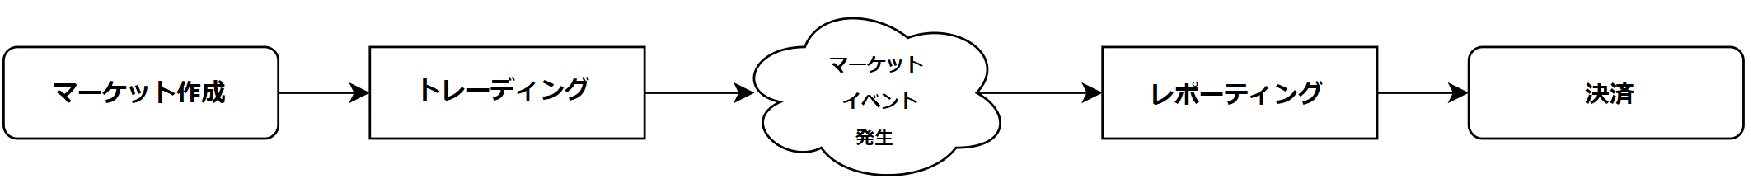
\includegraphics[bb=0 0 860 120, width=0.8\textwidth]{overview.pdf}
\caption{予測市場のライフタイム概要}
\label{fig:overview}
\end{figure*}

\subsection{マーケット作成}

Augurではこれから起こるイベントについてのマーケットを作成することができる。\textit{マーケット作成者(maket createor)}は、\textit{イベント終了日時(event end time)}を設定し、イベントのアウトカムをレポートするための\textit{指名レポーター(designated reporter)}を選択する。指名レポーターはマーケットのアウトカムを一方的に決定するものではない。コミュニティには、指名レポーターのレポート内容に対して争議を行い、訂正する機会が常に与えられる。

次に、マーケット作成者はレポーターがアウトカムを決定するために使用する\textit{判決ソース(resolution source)}を選択する。判決ソースは単に「一般常識」でも良く、例えば、「米国エネルギー省」、\texttt{bbc.com}、特定のAPIエンドポイントのアドレス等の特定のソースでも良い。\footnote{例えば、「WeatherUndergroundで報告された、2018年4月10日のサンフランシスコ国際空港の最高気温(華氏)は?」というマーケットがあり、判決ソースとして\texttt{https://www.wunderground.com/history/airport/KSFO/2018/4/10/ DailyHistory.html}を指定している場合、レポーターはそのURLにアクセスし、表示されている最高気温をレポートすれば良い。}そして、トレーダーの決済時にマーケット作成者に対して支払われる\textit{作成者手数料(creator fee)}の設定を行う(手数料についての詳細は\ref{section:settlement}を参照)。最後に、マーケット作成者は2つの保証金を支払う。\textit{有効性保証金(validity bond)} と \textit{指名レポート不参保証金(designated report no-show bond)}(略して、\textit{不参保証金(no-show bond)})である。

有効性保証金の支払いはETHで行われ、この保証金はマーケットが\textit{無効(invalid)}以外のアウトカムになればマーケット作成者へ返却される。\footnote{無効マーケット(invalid market)とは、マーケット作成者が列挙したアウトカムのいずれも誤っているため、あるいはマーケットの文言が曖昧または主観的であるため、レポーターによって無効と判断されたマーケットのことである。\ref{section:ambiguous_or_subjective_markets} を参照}
有効性保証金は、明瞭なアウトカムがあり、明確に定義されたマーケットを作成する動機付けとなる。有効性保証金の金額は、直近のマーケットで無効と判定されたマーケットの割合から動的に設定される。\footnote{詳細はAppendix.\ref{section:bond_size_adjustment_details_validity_bonds}を参照。}

不参保証金は、ETHによって支払われる\textit{不参gas保証金(no-show gas bond)}と、REPによって支払われる\textit{不参REP保証金(no-show REP bond)}の2つから構成される。これらの保証金は、そのマーケットの\textit{イベント終了日時}が過ぎた最初の3日以内に指名レポーターがレポートを行えば、マーケット作成者に返却される。3日以内に指名レポーターがレポートしなかった場合、マーケット作成者の不参保証金は没収され、\textit{ファーストパブリックレポート(first public report)}でレポートをしたレポーターにその保証金が与えられる(セクション\ref{section:open_reporting}を参照)。これにより、マーケット作成者は信頼性の高い指名レポーターを選択する動機付けとなり、マーケットの判決も早く下される。

不参gas保証金は、ファーストパブリックレポーターのgasコストを賄うために設けられた。この保証金によって、ファーストパブリックレポーターのgasコストが高すぎるためにレポーターに損益が出る、という事態を防いでいる。不参gas保証金は、直前の\textit{手数料期間(fee window)}の平均gasコストの2倍が設定される。

指名レポートが行われなかった場合、不参REP保証金は、ファーストパブリックレポーターがレポートしたアウトカムへの追加ステークという形で与えられる。ゆえに、不参REP保証金を受け取ることができるのは、ファーストパブリックレポーターが正しいレポートを行った場合のみである。有効性保証金と同様、直前の手数料期間にレポートを行わなかった指名レポーターの割合に応じて、不参REP保証金の金額は調整される。\footnote{詳細はAppendix.\ref{section:bond_size_adjustment_details_no-show_bonds}を参照。}

これら一連のマーケット作成とそれに伴う必要な保証金の支払いは、単一のEthereumトランザクションで行われる。このトランザクションが承認されれば、マーケットでのトレードが開始される。

\subsection{トレーディング}

マーケット参加者は、アウトカムの\textit{シェア(shares)}を取引することにより、そのイベントのアウトカムを予測する。\textit{シェアのコンプリートセット(complete set of shares)}は、そのイベントで有効なアウトカムに該当するシェアの集合で構成される~\cite{Clark_2014}。コンプリートセットは、トレードを完了させるためAugurのコントラクト上にあるマッチングエンジンによって必要に応じて作成される。

例えば、\texttt{A}、\texttt{B}の2つのアウトカムが予想されるマーケットを考えてみよう。アリスは\texttt{A}のシェアに0.7ETHを支払い、ボブは\texttt{B}のシェアに0.3ETHを支払うとする。\footnote{リリース初めは、AugurのマーケットではEthereumのネイティブこいんであるEther(ETH)が使用可能である。続くリリースで、Ethereumネットワーク上で発行された任意のトークンをサポートし、法定通貨に固定されたトークン("stablecoin")と同様、他マーケットのシェアも取り扱う予定である。} まず、Augurはこれらのオーダーをマッチングし、アリスとボブから合計1ETHを受け取り\footnote{ここでは、説明を簡単にするために1桁の数字である1ETHを使用している。実際のシェアのコンプリートセットのコストはこれよりもはるかに小さい。詳細は\texttt{docs.augur.net/\#number-of-ticks}を参照。\label{footnote:complete_set_cost}}、シェアのコンプリートセットを作成して、アリスに\texttt{A}のシェア、ボブに\texttt{B}のシェアを与える。こうして各アウトカムのシェアが生成される。シェアが生成されれば、あとは自由に取引することができる。

Augurのトレード用コントラクトは、プラットフォーム上に作成された全てのマーケットのオーダーブックを保持している。新しいオーダーは誰でも作成でき、存在するオーダーに対していつでも約定することが可能である。オーダーはAugurのスマートコントラクト内にある自動マッチングエンジンにより約定される。シェアの売買要求は、オーダーブックにマッチングするオーダーが存在するならば即座に約定する。それは、既存のコンプリートセットのクローズ、または、新たなコンプリートセットの発行を含め、他参加者によるシェアの購入や売却によって遂行される。Augurのマッチングエンジンは、最悪の事態に備え、最小限のシェア、及び/または、キャッシュのみをマッチングに使用する。マッチングするオーダーが無い、または、部分的にしかオーダーを約定することができない場合、残りのオーダーは新しいオーダーとしてオーダーブックに置かれる。

オーダーはトレーダーが設定した制限価格よりも悪い価格で約定することはないが、より良い価格で約定することはある。未約定のオーダーと一部約定済みのオーダーは、オーダー作成者によりいつでもオーダーブックから削除できる。手数料は、シェアのコンプリートセットが売却された場合にのみトレーダーにより支払われる。決済手数料については、セクション\ref{section:settlement}でより詳細に述べている。

シェアのトレードの大部分はマーケット決済前に行われると予想されるが、シェアはマーケット作成後であればいつでもトレード可能である。Augur上のすべての資産 -- アウトカムのシェア、パーティシペーショントークン、争議保証金のシェア、さらにはマーケット自体の所有権までも -- は(トークン化されているという意味で)常に譲渡可能である。

\subsection{レポーティング}\label{section:reporting}

マーケットのイベント発生後は、ファイナライズし決済を開始するためにアウトカムを決定しなくてはならない。アウトカムは、Augurのオラクル(現実に起きた事実をレポートすることで利益を得る、レポーターと呼ばれる人々で構成)によって決定される。REPを所有する人は誰でも、アウトカムに対してレポーティングや争議を行うことができる。レポートがコンセンサスに合致していれば、レポーターは報酬を得られるが、合致しなければ罰金を科せられる(セクション\ref{section:rep_redistribution}参照)。

\subsubsection{手数料期間}

Augurのレポーティングシステムは、7日間の\textit{手数料期間(fee windows)}が繰り返されることにより稼働する。手数料期間中にAugurによって収集された全ての手数料は、\textit{レポーティング手数料プール(reporting fee pool)}に加算される。手数料期間の最後に、レポーティングに参加したREP保有者に対し、このレポーティング手数料プールから支払いが行われる。レポーターは手数料期間中にステークしたREPの量に比例して報酬を受け取る。ここで言うレポーティングへの参加とは、イニシャルレポートでREPをステークすること、暫定アウトカムに対して争議すること、\textit{パーティシペーショントークン(participation tokens)}を購入することを指す。

\subsubsection{パーティシペーショントークン}

手数料期間中、REP保有者は 1 attorep\footnote{1 \textit{attorep} は $10^{-18}$ REP。}単位で、任意の数のパーティシペーショントークンを購入できる。手数料期間の最後に、購入したパーティシペーショントークンはREPに戻して返却され、さらに、購入したパーティシペーショントークン量に応じて、レポーティング手数料プールから手数料を獲得することができる。もし、レポーターが求められる行為(\textit{例}:レポート提出、別ユーザーのレポートに対する争議)を行わない場合は、パーティシペーショントークンを購入することで、手数料期間中にAugurに姿を現すことを意思表示できる。REPをステークすることと同様、パーティシペーショントークンの所有量に応じて、手数料期間に収集された手数料を獲得できる。

セクション\ref{section:incentives_and_security}で述べているように、REP保有者がマーケットのフォークへの参加に備えていることは重要である。パーティシペーショントークンは、REP保有者に少なくとも週に一度プラットフォームを監視する動機づけとなるため、その必要性が生じた場合は参加の促進に繋がる。パーティシペーショントークンを購入して手数料を手に入れる、というインセンティブがあるため、レポーティングへの参加を望まないREP所有者に対しても、手数料期間の七日間に一度はAugurにチェックインさせる動機づけとなる。この定期的なチェックインは、Augurの利用促進、フォーク発生検知の促進となり、結果、フォークが発生した場合にユーザーの参加が促進される。

\subsubsection{マーケットの状態の進行}

Augurのマーケットは作成後に7つの状態に遷移する。Augurのマーケットの潜在的な状態、すなわち「フェーズ」は次の通り
\begin{itemize}
\item レポーティング前
\item 指名レポーティング
\item 公開レポーティング
\item 次の手数料期間開始待ち
\item 争議ラウンド
\item フォーク
\item ファイナライズ
\end{itemize}

これらの状態の関係をFigure.~\ref{fig:reporting}に示す。

\begin{figure*}
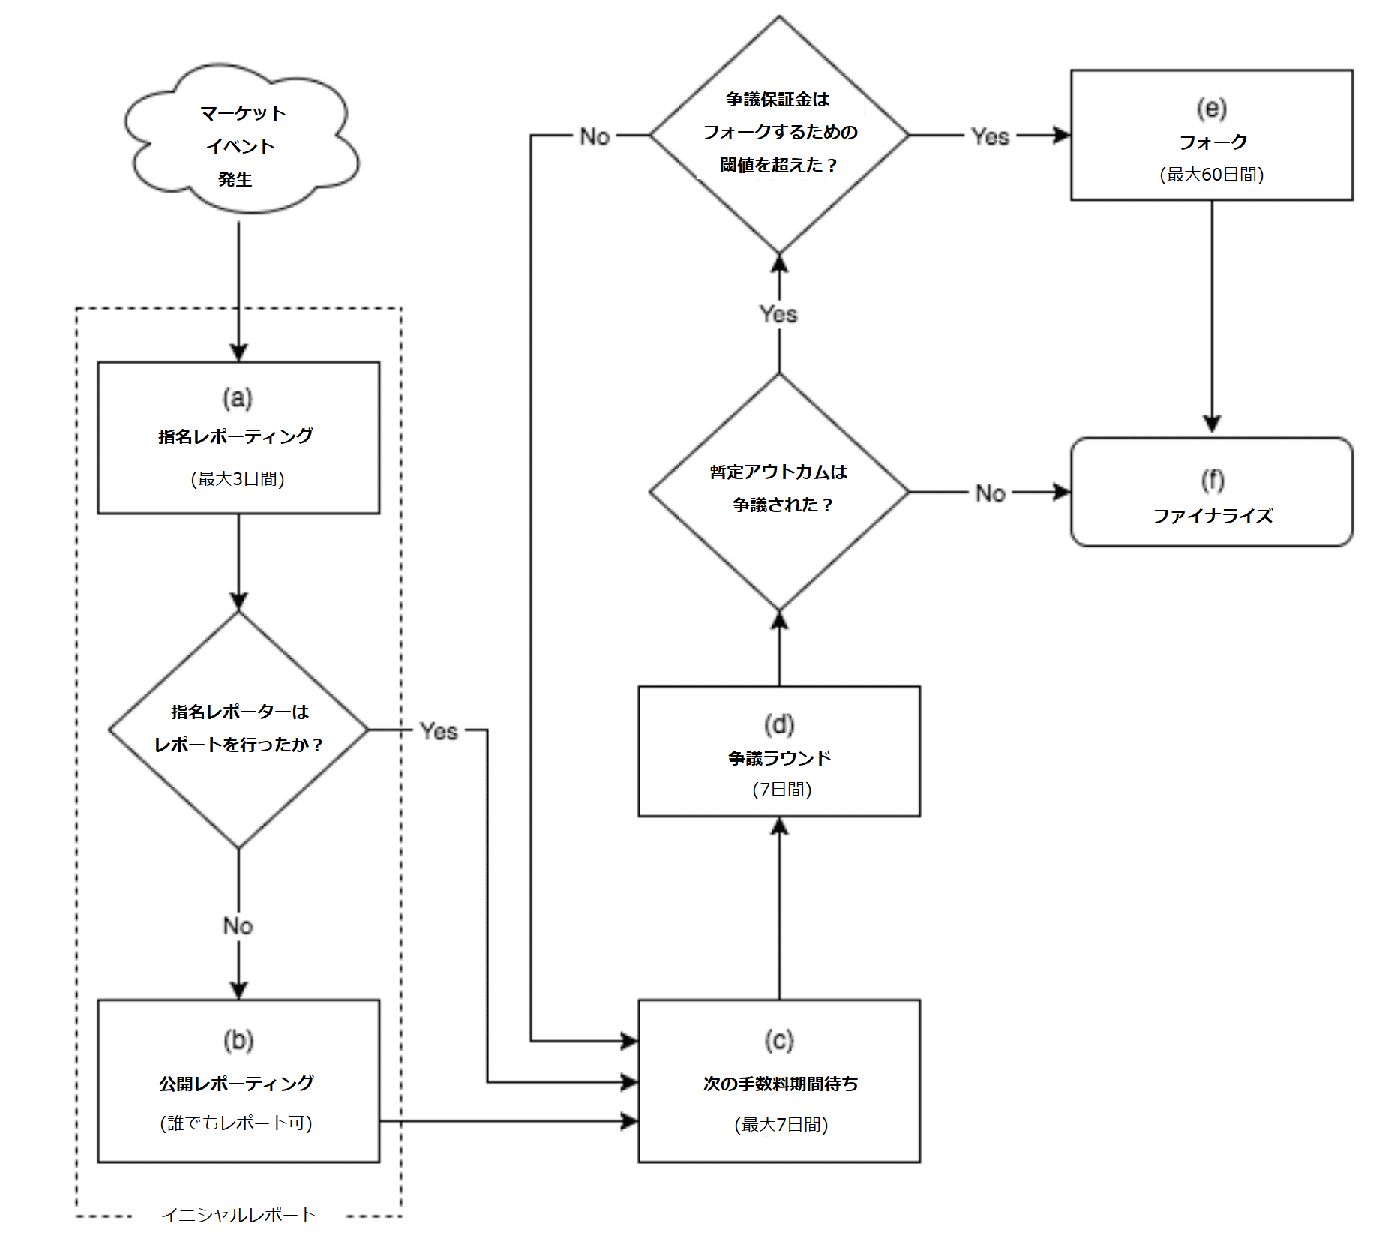
\includegraphics[bb=0 0 621 596, width=0.8\textwidth]{new_reporting.pdf}
\caption{レポーティングフローチャート}
\label{fig:reporting}
\end{figure*}

\subsubsection{レポーティング前}

\textit{レポーティング前(pre-reporting)}、または\textit{トレーディング(trading)}フェーズ(Figure.~\ref{fig:overview})とは、トレード開始からマーケットのイベントが発生するまでの期間を指す。一般に、Augurのマーケットにおいて最も活発にトレードが行われる期間である。マーケットがイベント終了日時を過ぎると、\textit{指名レポーティング(Designated Reporting)}フェーズに突入する(Figure.~\ref{fig:reporting}a)

\subsubsection{指名レポーティング}

マーケット作成時、作成者は指名レポーターを選び、不参保証金を支払う必要がある。指名レポーティングフェーズ(Figure.~\ref{fig:reporting}a)では、指名レポーターはイベントのアウトカムをレポートするために3日間の猶予が与えられる。指名レポーターがその3日以内にレポートしなかった場合、マーケット作成者は不参保証金を失い、マーケットは自動的に\textit{公開レポーティング(Open Reporting)}フェーズに移行する(Figure.~\ref{fig:reporting}b)。

指名レポーターがその3日以内にレポートを行えば、不参保証金はマーケット作成者に返却される。指名レポーターは自身がレポートしたアウトカムに対して、指名レポーターステーク\footnote{指名レポーターステークの大きさについての詳細はAppendix.\ref{section:bond_size_adjustment_details_designated_reporter_stake}を参照}を支払う必要があり、仮に指名レポーターがレポートした以外のアウトカムにマーケットがファイナライズすると、指名レポーターステークは没収される。\footnote{没収されたステークは、該当の手数料期間のレポーティング手数料プールに加算され、真実をレポートしたレポーターや争議を行った者への報奨金として使用される。詳細はセクション\ref{section:rep_redistribution}を参照。}指名レポーターがレポートを行うとすぐにそのマーケットは\textit{次の手数料期間開始待ち(Waiting for the Next Fee Window to Begin)}フェーズに移行し(Figure.~\ref{fig:reporting}c)、指名レポーターがレポートしたアウトカムはそのマーケットの\textit{暫定アウトカム(tentative outcome)}となる。

\subsubsection{公開レポーティング}\label{section:open_reporting}

もし、指名レポーターが割り当てられた3日以内にレポートできなかった場合、マーケット作成者は不参保証金を没収され、直後そのマーケットは\textit{公開レポーティング(open reporting)}フェーズに入る(Figure.~\ref{fig:reporting}b)。このフェーズでは、誰でもそのマーケットに対してレポートが可能となる。指名レポーターのレポート失敗後に最初にレポートを行ったレポーターを、そのマーケットの\textit{ファーストパブリックレポーター(first public reporter)}と呼ぶ。

ファーストパブリックレポーターは、彼らが選択したアウトカムへの追加ステークという形で、没収された不参保証金を獲得する。つまり、レポートしたアウトカムがマーケットのファイナルアウトカムになった場合にのみ、不参REP保証金を獲得することができる。不参gas保証金についても同様で、ファーストパブリックレポーターがレポートしたアウトカムがマーケットのファイナルアウトカムになった場合にのみ獲得できる。

ファーストパブリックレポーターはマーケットのアウトカムをレポートする際、(没収されている不参保証金がステークされているため)必ずしも所有するREPをステークする必要はない。このように、指名レポーターによるレポートが行われなかったマーケットは、公開レポーティングフェーズに入った瞬間誰かしらによって即時にレポートされることが期待できる。

\textit{イニシャルレポート(initial report)}がイニシャルレポーター(指名レポーター、あるいはファーストパブリックレポーター)によって行われると、そのアウトカムはマーケットの暫定アウトカムとなり、マーケットは次の手数料期間開始待ちフェーズへと移行する(Figure.~\ref{fig:reporting}c)。

\subsubsection{次の手数料期間開始待ち}

マーケットでイニシャルレポートが行われると、次の手数料期間開始待ちフェーズに入る(Figure.~\ref{fig:reporting}c)。このフェーズでは、現在の手数料期間が終了するまでレポーティングは保留状態となる。次の手数料期間が開始されると、マーケットは\textit{争議ラウンド(Dispute Round)}フェーズに入る。

\subsubsection{争議ラウンド}

争議ラウンド(Figure.~\ref{fig:reporting}d)は7日間あり、REP保有者であればマーケットの\textit{暫定アウトカム}に対して争議が行える。\footnote{争議ラウンドと手数料期間が同時期であるのは、純粋に便利性の問題である。原理的には、争議ラウンドと手数料期間の期間が異なることは可能である。}(争議ラウンド開始時の暫定アウトカムは、その後REP保有者による争議が無ければマーケットのファイナルアウトカムとなる)。争議とは、現在の暫定アウトカムとは異なるアウトカムにREPをステークすることである(このREPを\textit{争議ステーク(dispute stake)}と呼ぶ)。争議ステークの合計額が、争議ラウンドで必要な\textit{争議保証金額(dispute bond size)}に達すれば、その争議は成功である。争議保証金額は次のようにして導出される。

$A_n$を、$n$回目争議ラウンド開始時における、あるマーケットの全てのアウトカムの争議ステークの合計とする。$\omega$を、この争議ラウンド開始時における、あるマーケットの暫定アウトカム以外のアウトカムとする。$S(\omega, n)$を、$n$回目争議ラウンド開始時における、$\omega$に対する争議ステークの合計とする。すると、$n$回目争議ラウンドで、暫定アウトカムに対抗してアウトカム$\omega$で争議を成功させるために必要な\textit{争議保証金額}は次の式で求められる。
\beq \label{eq:bond_size}
B(\omega, n) = 2A_n - 3S(\omega, n)
\eeq

争議保証金額をこのように設定した理由は、事実と異なるアウトカムに対して争議を行い、その結果争議を成功させたレポーターに対し見返りとして50\%のROIを保証するためである(セクション\ref{section:leveraging_the_threat_of_a_fork}を参照)。

争議保証金は、必ずしも一人のユーザーが全額を払う必要はない。Augurのプラットフォームでは不特定多数のユーザーで争議保証金を募ることができる。誤った暫定アウトカムを見つけたユーザーは、暫定アウトカム以外のアウトカムにREPをステークすることで争議を発動できる。もし、いずれかのアウトカム(暫定アウトカム以外のアウトカム)の争議ステークが、争議保証金となりえる程十分に集まった場合、現在の暫定アウトカムに対する争議が成功したと言える。

争議が成功すると、マーケットは次の争議ラウンド、あるいは、\textit{フォーク(fork)}状態に移行する(Figure.~\ref{fig:reporting}e)。争議保証金額が全REPの2.5\%より大きくなると、マーケットはフォーク状態となる。争議保証金額が全REPの2.5\%より小さい場合は、争議のために新たに選択したアウトカムが暫定アウトカムとなり、マーケットは次の争議ラウンドに移行する。

争議ラウンド中、全ての争議ステークはエスクローで保持される。もし争議ステークが争議を成功させるだけの額に達しなかった場合、争議ステークは争議ラウンド終了時に争議ステークの所有者へ返却される。もし、7日間の争議ラウンドで争議が成功しなければ、マーケットは\textit{ファイナライズ(finalized)}状態となり(Figure.~\ref{fig:reporting}f)、その時の暫定アウトカムが\textit{ファイナルアウトカム}となる。つまり、マーケットのファイナルアウトカムとは、争議ラウンドを経たが争議失敗に終わった暫定アウトカム、または、フォークによって決定された暫定アウトカムのことである。Augurのコントラクトはこのファイナルアウトカムを\textit{真実(truth)}として扱い、それに従って支払いを行う。

争議に失敗した全ての争議ステークは、争議ラウンドが終了するたびに元の所有者へ返却される。争議に成功した全ての争議ステークは、支持したアウトカムに適用され、マーケットがファイナライズされるまで(または他のマーケットでフォークが発生するまで)その状態のままとなる。(争議の成功/失敗によらず)すべての争議ステークは、現在の手数料期間にある\textit{レポーティング手数料プール}\footnote{手数料期間中に収集された決済手数料と有効性保証金は、手数料期間のレポーティング手数料プールに加算される。手数料期間の最後に、レポーティング手数料プールから、手数料期間中にステークしたREP量に応じた額がユーザーに支払われる。}の一部を受け取る。

\subsubsection{フォーク}\label{section:fork}

フォーク状態(Figure.~\ref{fig:reporting}e)とは特殊な状態であり、最大60日間続く。フォークはマーケットの判決を下すための最終手段である。非常に破壊的なプロセスであり、発生することはほぼ無いと想定している。フォークが発生するのは、あるマーケットで争議保証金が全REPの2.5\%に達した場合である。このマーケットのことを、\textit{フォーキングマーケット(forking market)}と呼ぶ。

フォークが開始されると、その\textit{フォーキング期間(forking period)}は60日\footnote{フォーキング期間は60日間未満になることがある。フォーキング期間は、60日経過するか、全REPの50\%以上がチャイルドユニバースに移行すれば終了する。}続く。このフォーキング期間が終わるまで、ファイナライズされていない他の全マーケットは保留状態となる。REP保有者と(ウォレット、取引所などの)サービス提供者がフォークに対応する十分な時間が確保できるよう、フォーキング期間は通常の手数料期間よりも長く設定している。また、フォークで決定したファイナルアウトカムを争議することはできない。

全てのマーケットと全てのREPトークンは、\textit{ユニバース(universe)}に存在する。あるユニバースに存在するREPトークンは、同一のユニバースに存在するマーケットに対して\textit{のみ}、そのREPトークンでレポートを行うことができる(それにより手数料を獲得できる)。Augurがローンチされた直後、全てのマーケットと全てのREPは\textit{ジェネシスユニバース(genesis universe)}に存在する。

マーケットがフォークすると、新しいユニバースが生成される。フォークでは、フォーク対象のマーケットに存在するアウトカムの数だけ、新しい\textit{チャイルドユニバース(child universe)}が生成される(セクション\ref{section:settlement_of_invalid_markets}で述べているように、このアウトカムには\texttt{無効(Invalid)}を含む)。例えば、ある“バイナリ”マーケットでは、\texttt{A}、\texttt{B}、\texttt{無効}の3つのアウトカムがあるとする。このバイナリマーケットがフォークすると、ユニバース\texttt{A}、ユニバース\texttt{B}、ユニバース\texttt{Invalid} の合計3つのチャイルドユニバースが生成される。生成直後は、これらのユニバースは空の状態であり、マーケットやREPトークンは含まれていない。

フォークが開始されると、\textit{ペアレントユニバース(parent universe)}は永久的に\textit{ロック(locked)}される。ロック済みユニバースでは新しいマーケットを生成することはできない。ユーザーは、ロック済みユニバースにあるマーケットのシェアをトレードすることはでき、さらにイニシャルレポートも可能であるが、このユニバースではレポートに対する報酬は払われず、マーケットもファイナライズできない。ロック済みユニバース内のマーケットやREPトークンを利用可能にするためには、REPをいずれかのチャイルドユニバースに移行しなくてはならない。

ペアレントユニバースに存在するREPを保有するユーザーは、移行先のチャイルドユニバースを選択し、そのREPを移行することができる。移行は不可逆で一方向であるため、この選択は慎重に検討する必要がある。チャイルドユニバース間でのREPトークンのやり取りはできない。\textit{移行とは特定のマーケットのアウトカムに対するREPトークンの永久的なコミットメントである。}それぞれのチャイルドユニバースに移行されたREPトークンは、完全に分離されたトークンとみなすべきで、ウォレットや取引所などのサービス提供者もそのように取り扱うべきである。

フォークが開始すると、フォーキング期間中にチャイルドユニバースへの移行が自由に行えるように、フォーク対象でないマーケットにステークされている全てのREPは、そのステーク状態が\textit{解除(unstaked)}される。\footnote{唯一の例外は、イニシャルレポーターがイニシャルレポートでステークしたREPである。他マーケットでフォークが発生してもこのREPはアウトカムへのステーク状態が継続され、フォーク後に最もREPが移行されたチャイルドユニバースに自動的に移行される。}

フォーキング期間終了時に最もREPが移行されたチャイルドユニバースが\textit{ウィニングユニバース(winning universe)}となり、そのユニバースに対応するアウトカムがフォークしたマーケットのファイナルアウトカムとなる。ペアレントユニバースにあるファイナライズされていないマーケットは、このウィニングユニバースにのみ移行され、そこでイニシャルレポートが行われると、次の手数料期間開始待ちフェーズにリセットされる。

\paragraph*{ペアレントユニバースからチャイルドユニバースに対してトークンを移行させるにあたり、時間制限はない。}トークンはフォーキング期間後に移行されるが、これらのトークンはユニバースの勝利決定には影響を与えない。フォーキング期間中の参加を促進するため、フォーク開始から60日以内にREPを移行させた保有者すべてに、移行先のチャイルドユニバースで5\%のREPを追加付与する\footnote{これは、全体の50\%以上のREPがいずれかのチャイルドユニバースに移行したことにより、早期にフォーキング期間が終了した場合でも発生する。}。この報酬は新しいREPトークンを生成することによって支払われる。\footnote{このREP追加発行の効果は小さい。例えば、全体の20\%にあたるREPがフォーキング期間中に移行されたとして、これによる追加発行は全体の1%に過ぎず、加えてフォークは非常に稀なイベントと予想されるためである。}

\paragraph*{フォーク対象のマーケットのアウトカムに対してREPをステークしたレポーターは、フォーク中にそのポジションを変更することはできない。}ペアレントユニバースのアウトカムにステークされたREPは、そのアウトカムに対応するチャイルドユニバースにしか移行できない。例えば、争議ラウンドにおいて、あるレポーターがアウトカム\texttt{A}が正しいアウトカムだと信じ、アウトカム\texttt{A}に対する争議保証金を支払った場合、フォーク中はユニバース\texttt{A}にのみ、そのREPを移行することが可能である。

\paragraph*{シブリングユニバース(sibling universe)は完全に分離されている。}あるユニバースに存在するREPトークンで、別のユニバースにあるマーケットをレポートすることは不可能であり、それによって報酬を得ることもできない。ユーザーは、信用できないオラクルが存在するユニバースでのマーケット作成やトレードを望まないと想定されるため、事実にそぐわないユニバースではREPによって手数料を稼げる可能性は低くなる。その結果、そのユニバースの市場価値は大きくならないだろう。フォーク後、事実にそぐわないユニバースがウィニングユニバースになるか否かに関わらず、そのユニバースに移行したREPの市場価値は失われるだろう。このことはセキュリティ上重要な結論である。この件についてはセクション\ref{section:incentives_and_security}で考察している。

\subsubsection{ファイナライズ}

フォークが完了する、または、暫定アウトカムに対する争議が成功しない状態で争議ラウンドが7日経過すれば、そのマーケットはファイナライズ状態(Figure.~\ref{fig:reporting}f)に入る。フォークしたアウトカムに対して争議することは不可能であり、フォークしたアウトカムはフォーキング期間終了時にファイナライズしたとみなされ、トレーダーはすぐにそのマーケットでポジションを決済することができる。マーケットがファイナライズ状態になった時、選ばれたアウトカムを\textit{ファイナルアウトカム(final outcome)}と呼ぶ。

\subsection{マーケットの決済}\label{section:settlement}

トレーダーは次の2つの方法のいずれかによりポジションを決済することができる。一つは、所有するシェアを通貨と交換して他のトレーダーに売却する方法、もう一つは、所有するシェアをそのマーケットで決済する方法である。前述の、合計1ETHがAugur上でエスクロー取引された時にコンプリートセットの一部としてシェアが生成された例を思い出してほしい。\footref{footnote:complete_set_cost} エスクローから1ETH取り出すためには、トレーダーはAugurに対してコンプリートセットを提供するか、もしくはマーケットが既にファイナライズしているならば、ウィニングアウトカムのシェアをAugurに対して提供しなくてはならない。この交換が発生した時、\textit{トレーダーがマーケットコントラクトに対して決済した}、と言う。

例として、アウトカム\texttt{A}と\texttt{B}が存在する未ファイナライズのマーケットを考えてみる。アリスはアウトカム\texttt{A}のシェアを保有しそれを0.7ETHで売却したいと希望しており、ボブはアウトカム \texttt{B}のシェアを保有しそれを0.3ETHで売却したいと希望しているとする。まずAugurはこれらのオーダーをマッチングし、参加者から\texttt{A}と\texttt{B}のシェアを収集する。その後Augurはアリスに0.7ETH(実際はここから手数料が差し引かれる)を与え、ボブに0.3ETH(同様に手数料が差し引かれる)を与える。

二つ目の例として、ウィニングアウトカムが\texttt{A}とファイナライズされたマーケットを考えてみる。アリスはアウトカム\texttt{A}のシェアを保有しその換金を希望している。アリスはそのアウトカム\texttt{A}のシェアをAugurに送り、1ETH(手数料が差し引かれる)を受け取る。

\subsubsection{決済手数料}

Augurでは、参加者がマーケットコントラクトに対して決済した時にのみ手数料が課せられる。課せられる手数料は、作成者手数料とレポーティング手数料の2つである。これらの手数料は両方とも決済した額に比例する。従って、アリスが0.7ETH、ボブが0.3ETH受け取った上記の未ファイナライズマーケットの例では、アリスは手数料の70\%、ボブは手数料の30\%を支払う。

作成者手数料はマーケット作成時に作成者により設定され、決済時にそのマーケット作成者に支払われる。レポーティング手数料は動的に設定され(セクション\ref{section:market_cap_nudges}参照)、レポーティングに参加したレポーターに支払われる。

\subsubsection{無効マーケットの決済}\label{section:settlement_of_invalid_markets}

ファイナルアウトカムが\texttt{無効}となったマーケットでは、マーケットコントラクトに対して決済を行ったトレーダーは各アウトカムのシェア毎で同額のETHを受け取る。つまり、もし$N$個のアウトカム(無効は含まない)があり、シェアのコンプリートセットの金額が$C$ ETHだとすると、トレーダーは一つのシェアで$C/N$ ETHを受け取る。\footnote{もしマーケットのアウトカムが\texttt{無効}でファイナライズした場合、技術的制約があるためトレードを簡単に取引前の状態に巻き戻すことはできない。アウトカムのシェアはただのトークンであり、ユーザー間で直接取引することができる。つまり、ETHとシェアはAugurの制御配下に無く、マーケットが\texttt{無効}にファイナライズしたからといって、これらを元の所有者に返却することはできない。}

\subsubsection{Reputationの再配布}\label{section:rep_redistribution}

マーケットがフォークすることなくファイナライズした場合、ファイナルアウトカム以外にステークされた全てのREPは没収され、その没収されたREPは、ファイナルアウトカムにステークした各ユーザーに対して、そのステークしたREP量に応じて再配布される。争議保証金額は、争議でファイナルアウトカムとなるアウトカムに争議ステークとしてステークされたREPが、報酬としてROIが50\%となるように決定される。\footnote{Appendix.\ref{section:finalization_time}の定理\ref{th:roi_guarantee}参照。}この報酬は、現実の結果にそぐわない暫定アウトカムがあった場合に、レポーターが争議を発動させるための強いインセンティブとなる。

\section{インセンティブとセキュリティ}\label{section:incentives_and_security}

REPの時価総額とAugurのフォーキングプロトコルの信頼性の間には、強い関係性がある。REPの時価総額が十分に大きく\footnote{詳細はセクション\ref{section:integrity_forking_protocol}参照。}、攻撃者が経済的合理性を有する場合、フォークで勝利したアウトカムは客観的現実と合致するものになるはずである。実際には、指名レポーターや争議ラウンドの仕組みを使わなくてもAugurは適切に機能するであろうし、フォーキングプロセス\textit{さえ}あればオラクルは誠実にレポートを行うだろう。

しかし、フォークは破壊的であり時間を浪費する。フォークは一つのマーケットで判決を下すまで最大60日かかり、さらに1度に1つのマーケットにしか処理できない。フォーク中のマーケットが判定される60日の間、ファイナライズされていない他の全マーケットは保留状態となる。\footnote{トレーダーはこれらのマーケット上でトレードを続行することはできるが、マーケットのファイナライズはフォーキング期間が終わるまでできない。}サービス提供者はサービスの更新が必要となり、REP保有者はREPを新しいチャイルドユニバースに移行する必要がある。それゆえ、フォークは絶対に必要な場合のみ実施されるべきである。言うなれば、フォークの実行は核兵器を使用するようなものである。

首尾よく、フォークは真実を決定するために信頼できるものであるということが定着すれば、実際にフォークせずともインセンティブによって参加者を正直に行動するよう促すことができる。\textit{フォークとは信頼できる脅威であり、フォークが正しい判決を下すという信念は、Augurのインセンティブシステムの基盤となっている。}

次に、フォーキングシステムが真実を決定できるための要件について説明する。ここでは、インセンティブシステムと、そのインセンティブシステムが如何にして迅速かつ正確に全マーケットの判決を下すことを促進するかを考察する。

\subsection{フォーキングプロトコルの完全性}\label{section:integrity_forking_protocol}

ここではフォーキングプロセスの確実性と信頼可能となる条件について説明する。以下では説明を簡単にするために、フォークについて言及する場合、チャイルドユニバースは客観的現実に合致した、\texttt{トゥルー(true)}ユニバースとし、それ以外のチャイルドユニバースは事実とは異なる、\texttt{フォルス(false)}ユニバースとする。また、最もREPが移行されるチャイルドユニバースをウィニングユニバースとし、それ以外のチャイルドユニバースは\textit{ルージングユニバース(losing universe)}とする。

当然、我々は\texttt{トゥルー}ユニバースがウィニングユニバースとなり、\texttt{フォルス}ユニバースはルージンズユニバースになることを望んでいる。仮にフォーキングプロトコルへの攻撃が成功し、その結果、フォルスユニバースがウィニングユニバースになってしまった場合、そのフォーク対象のマーケットから(潜在的には未ファイナライズのマーケットからも)不正な支払いが行われることになるだろう。

我々は、攻撃するために必要となる最低限のコストよりも、攻撃の成功により得られる最大利益を小さくすることで、オラクルを保護しようと取り組んでいる。このことを以下に成文化する。

\subsubsection{攻撃者の最大利益}

オラクルへの攻撃が成功した場合、未ファイナライズのマーケットは\texttt{フォルス}ユニバースに移行される。もし攻撃者が\texttt{フォルス}ユニバースで大多数のREPをコントロールできるのであれば、未ファイナライズのマーケットを思い通りの判決結果にすることができる。最も極端なケースでは、未ファイナライズマーケットでエスクロー取引されている資金全てを攻撃者が獲得することとなる。\footnote{攻撃者はいくつかのアウトカムの\textit{全ての}シェアを獲得し、強制的にマーケットをそのアウトカムにファイナライズする必要がある。}

\begin{definition}
Augurの未ファイナライズなマーケット内でエスクローされている資金の合計額を、Augurの\textit{ネイティブ未決済建玉(native open interest)}と定義し、$I_a$で示す。 \footnote{これにはAugurへレポーティング手数料を支払う外部市場が含まれる。}
\end{definition}

\begin{definition}
Augurに対して一切レポーティング手数料を支払わないが、Augurのマーケットの判決結果に従い、自身のマーケットの判決を下すマーケットのことを、\textit{寄生的マーケット(parasitic market)}と定義する。
\end{definition}

\begin{definition}
 Augurのマーケットに連動して判決を下す寄生的マーケットでエスクローされている資金の合計額を、\textit{寄生的未決済建玉(parasitic open interest)}と定義し、それを$I_p$で示す。
\end{definition}

最も極端なケースでは、攻撃者は全寄生的マーケットの全資金を獲得可能である。

\begin{observation}
オラクルへの攻撃が成功した攻撃者の最大利益(グロス値)は、$I_a + I_p$である。
\end{observation}

\subsubsection{寄生的未決済建玉の不可知性}

Augurの$I_a$を正確かつ効率的に測定することは可能である。しかし、一般に$I_p$は不可知である。なぜならば、オフラインな寄生的マーケットはランダムに多数存在し、それらのマーケットの未決済建玉の額もまたランダムであるためである。攻撃者の最大利益に不可知な値である$I_p$を含むため、オラクルは経済的合理性を持つ者からの攻撃に対して安全であるという客観的な確信を得ることは不可能である。

しかし、実際には$I_p$に合理的制限があると仮定すれば、オラクルは安全であるという条件を定義できる。

\subsubsection{攻撃成功のための最小コスト}

次に、オラクルを攻撃するためのコストについて考察する。REPの価格を$P$とする。attorepを$\epsilon$とする\footnote{1 \textit{attorep}は$10^{-18}$ REP。}。現存するREPの総量(REPの``マネーサプライ“)を$M$とする。フォーキング期間中にトゥルーユニバースに移行される$M$の割合を$S$とする。

すると、積$SM$はフォーキング期間中にトゥルーユニバースに移行するREPの総量となり、さらに積$PM$はREPの時価総額となる。

攻撃者が選択した\texttt{フォルス}ユニバースに対して移行したREPの価格を$P_f$とする。$P \leq P_f$ の場合、REPを移行しないことよりも、REPを\texttt{フォルス}ユニバースに移行することの方が有益となるため、オラクルは経済的合理性を持つ攻撃者に対して安全とは言えない。

\subsubsection{完全性}

\begin{assumption}
攻撃者でないレポーターは、フォーク中に\texttt{フォルス}ユニバースにREPを移行しないものとする。\footnote{偶然や不注意によって、悪意のないレポーターが\texttt{フォルス}ユニバースにREPを移行する可能性はあるが、そのレポーターが攻撃者の共犯者か否かは判別できない。}
\end{assumption}

設計上、オラクルに対する攻撃を成功させるには、フォーキング期間中に\texttt{トゥルー}ユニバースよりも多いREPを\texttt{フォルス}ユニバースに移行する必要がある。仮定より、攻撃者のみが\texttt{フォルス}ユニバースにREPを移行したとする。すると、フォーキング期間中に\texttt{トゥルー}ユニバースに移行されたREP量は、$SM$で示すことができる。従って、攻撃を成功させるためには、少なくとも$SM + \epsilon$ REPを移行する必要がある。単純化するため$\epsilon$は無視できる程小さい値とすると、攻撃を成功させるためには少なくとも$SM$ REPを、\texttt{フォルス}ユニバースに移行する必要がある。

攻撃者がフォーキング期間中に$SM$ REPを移行した場合、攻撃者は移行先であるチャイルドユニバースで$SM$ REPを受け取ると考えられる。\footnote{実際には、フォーク開始から60日以内に移行するとボーナスとして5\%付与されるため、チャイルドユニバースで受け取るREPは、$1.05 SM$ REPとなる。ここでは考察を簡単にするため、5\%のボーナスは無視する。詳細はAppendix.\ref{ap:early_migration_integrity}を参照。}もし、攻撃者が\texttt{フォルス}ユニバースに移行したとすると、それらのコインの価値は$SMP_f$となる。故に、攻撃の成功に必要な最小コストは$(P - P_f)SM$である。


\begin{observation}
フォーク中に、攻撃者がフォルスユニバースに移行するREPの最小量は$SM$であり、その移行には$(P - P_f)SM$のコストがかかる。
\end{observation}

$S > \frac{1}{2}$の場合は、フォルスユニバースがウィニングユニバースとなるための十分なREPが\texttt{トゥルー}ユニバース以外のユニバースに存在しないため、攻撃は不可能である点に注意してほしい。

経済的合理性のある攻撃者に対抗するため、攻撃の成功に必要な最小コストよりも最大利益の方が小さい場合、オラクルは客観的現実に一致するアウトカムを選択するだろう。観察1、2より、$S > \frac{1}{2}$、または、$I_a + I_p < (P - P_f)SM$ を満たす限り、必ずこの状況となる。このことから以下の完全性の公式定義が得られる。


\begin{definition}\label{ob:integrity_property}
(完全性の性質) フォーキングプロトコルは、$S > \frac{1}{2}$、または、$I_a + I_p < (P - P_f)SM$、であれば常に完全性がある。
\end{definition}

上記の不等式から、フォーキングプロトコルの完全性とREPの時価総額$PM$の関係性を求めることができる。

\begin{theorem}\label{th:market_cap_security_theorem}
(時価総額の安全性定理) フォーキングプロトコルに完全性があるための必要十分条件は、以下である。
\begin{enumerate}
\item $S > \frac{1}{2}$、または
\item $P_f < P$、かつ、REPの時価総額が $\frac{(I_a + I_p)P}{(P - P_f)S}$ より大きい。
\end{enumerate}
\end{theorem}

\begin{proof}
フォーキングプロトコルに完全性があると仮定すると、定義より、$S > \frac{1}{2}$ または $I_a + I_p < (P - P_f)SM$ である。$I_a + I_p < (P - P_f)SM$ とすると、$I_a + I_p \geq 0$ かつ $SM > 0$ であるため、 $P_f < P$ である. $I_a + I_p < (P - P_f)SM$ より $PM$ を求めると、 $\frac{(I_a + I_p)P}{(P - P_f)S} < PM$ となり、一方向目が証明された.

次に、$S > \frac{1}{2}$、または、$P_f < P$ かつ $\frac{(I_a + I_p)P}{(P - P_f)S} < PM$ とする。 $S > \frac{1}{2}$の場合、定義よりフォーキングプロトコルに完全性がある。さらに、$P_f < P$ かつ $\frac{(I_a + I_p)P}{(P - P_f)S} < PM$ の場合、$I_a + I_p$ を求めると、$I_a + I_p < (P-P_f) SM$ となるため、逆方向も証明された。
\end{proof}

\subsection{仮定とその帰結}

トレーダーは、虚偽のレポートが行われるユニバースではトレードを望まないと考えられる。また、マーケット作成者は、トレーダーが存在しないユニバースではマーケットの作成を望まないと考えられる。このようなマーケットやトレードが存在しないユニバースでは、REP保有者に対していかなる配当も提供されない。故に、\texttt{フォルス}ユニバースに移行されたREPは市場価値を失い、これを $P_f = 0$ でモデル化する。

フォーキング期間中に、存在するREPの少なくとも20\%は\texttt{トゥルー}ユニバース移行すると考えられるため、これを $S \geq \frac{1}{5}$ でモデル化する。また、ネイティブ未決済建玉の50\%に及ぶ寄生的未決済建玉に対応するため、$I_a \geq 2 I_p$ とする。

これらの前提の下、定理\ref{th:market_cap_security_theorem} より、REPの時価総額がネイティブ未決済建玉の7.5倍以上であれば、フォーキングプロトコルに完全性があるといえる。\footnote{代替的な仮説とその帰結については、Appendix.\ref{section:alternative_assumptions}参照。}

\subsection{時価総額ナッジ}\label{section:market_cap_nudges}

AugurはREPの価格に関する情報を、現実世界で起こる他の情報と同じ手法、つまりAugurのマーケットから取得する。これにより、Augurは自身でREPの時価総額を算出することができる。また、Augurは現在のネイティブ未決済建玉を取得することもできるため、Augurの完全性要件を満たすための時価総額が決定できる。

全てのユニバースにおいて、そのユニバース開始時のレポーティング手数料は1\%である。もし現在の時価総額が目標値よりも低い場合、レポーティング手数料は自動的に増加する(ただし33\%を超過することはない)ことで、REPの価格に対して上昇圧力を、新たなネイティブ未決済建玉に対しては下降圧力をかける。反対に、現在の時価総額が目標値よりも高い場合、トレーダーがシステムを安全に保つための手数料を必要以上に支払わなくていいよう、レポーティング手数料は自動的に減少する(ただし0.01\%を下回ることはない)。

レポーティング手数料は次のようにして決定する。直前の手数料期間でのレポーティング手数料を $r$、目標の時価総額を $t$ 、現在の時価総額を $c$ とすると、現在の手数料期間のレポーティング手数料は、$\max\left\{ \min\left\{\frac{t}{c}r, \frac{333}{1000}\right\} , \frac{1}{10,000}\right\}$となる。

\subsection{フォークの脅威を活用する}\label{section:leveraging_the_threat_of_a_fork}

前述したように、フォークとは破壊的でマーケットをファイナライズするためには時間を要する。全てのマーケットをフォークで判決するのではなく、フォークの\textit{脅威}を有効に活用してマーケットの判決を行う。

争議でファイナルアウトカムに賛成票を投じた場合、争議ステークに対して50\%のROIが報酬として得られることを思い出してほしい。\footnote{ファイナルアウトカムに一致するユニバースに存在するREPで測定される件については、Appendix.\ref{section:finalization_time}の定理\ref{th:roi_guarantee}を参照。}フォーク発生時、事実と異なるアウトカムにステークされたREPは無価値となり、反対に、事実と一致するアウトカムにステークされたREPはチャイルドユニバースで50\%以上のREPが報酬として与えられる。それゆえにフォークに突入すれば、事実と異なるアウトカムを争議して正しいアウトカムに賛成票を投じたREP保有者は常には優位性があり、事実と異なるアウトカムに賛成票を投じたREP保有者のREPは経済的価値を失うだろう。

我々は、このような背景から、事実と異なる全ての暫定アウトカムは必ず争議の対象になると確信している。

\section{潜在的問題と危険性}

\subsection{寄生的マーケット}
寄生的マーケットとは、Augurに対してレポーティング手数料の支払いはないが、ネイティブなAugurのマーケットの判決結果に従い判決を下すマーケットであった。寄生的マーケットは手数料の支払い対象となるレポーターは存在せずにAugurと同様のサービスを低い手数料で提供できる。これはフォーキングプロトコルの完全性に深刻な影響を及ぼす可能性がある。
特に、Augurにあったトレードの関心を寄生的マーケットが奪う場合、Augurのレポーターが受け取るレポーティング手数料は少なくなるだろう。これはREP時価総額の下降圧力となる。REP時価総額が低すぎるとフォーキングプロトコルの完全性は危険にさらされる(定理\ref{th:market_cap_security_theorem})。その結果、寄生的マーケットはAugurの長期生存性を脅かす可能性があり、Augurはこのことには激しく抵抗しなくてはならない。

この寄生的マーケットに対する最善の防衛策の一つは、Augur上で寄生的マーケットを稼働させた際の報酬を最小限に抑えるために、(オラクルの完全性を持続させつつも)プラットフォームであるAugurでのトレーディングをできるだけ安くすることである。

\subsection{未決済建玉のボラティリティ}
ポピュラーなスポーツイベント期間中にみられるような、大きく、急で、予測できない未決済建玉の増加は、フォーキングプロトコルの完全性の要件である時価総額の急激な増加につながる(定理\ref{th:market_cap_security_theorem})。その時点の時価総額が時価総額要件に満たない場合、経済的合理性を持つ攻撃者によって誤った判決に導くためのフォークが引き起こされる危険性がある。これを防ごうとAugurは時価総額を上昇させようと試みるが(セクション\ref{section:market_cap_nudges}参照)、これらの試みは反動的であり7日間の手数料期間毎に1回しか調整されない。

しかしながら注目すべき点は、未決済建玉の急激な増加を目の当たりにしている投機家は、この時価総額の反動ナッジを見越してREPを購入する可能性があり、その結果、おそらくフォーキングプロトコルの完全性が脅かされなくなるまで時価総額が上昇する。従って、攻撃者はオラクルの脆弱な期間を利用して攻撃を成功させるだけの十分な時間は取れないだろう。

\subsection{不整合あるいは悪意のある判決ソース}

マーケット作成時、作成者はレポーターがアウトカムを決定するための判決ソースを選択する。もしマーケット作成者が不整合または悪意のある判決ソースを選択した場合、正直なレポーターは資金を失う可能性がある。

例えば、セレナというマーケット作成者が、アウトカム\texttt{A}、\texttt{B}の2つあるマーケットを作成し、判決ソースとして彼女のウェブサイト\texttt{attacker.com}を選択、指名レポーターに彼女自身を設定したとする。マーケットのイベント終了後、指名レポーターである彼女はアウトカム\texttt{A}をレポートし、\texttt{attacker.com}の内容をアウトカム\texttt{B}が正しいアウトカムであるかのように書き換える。正直なレポーターは\texttt{attaker.com}をチェックするとイニシャルレポートが正しくないと認識した後、最初の争議ラウンドで暫定アウトカムに対する争議を起こし、その争議の結果、首尾よくアウトカムBが正しいという結果になったとする。その後セレナは\texttt{attacker.com}の内容をアウトカム\texttt{A}が正しいアウトカムであるかのように書き換え、マーケットは2回目争議ラウンドに突入する。再度、レポーターは\texttt{attacker.com}をチェックし、暫定アウトカムであるアウトカム\texttt{B}は正しくないと認識するため、その争議は成功し、アウトカム\texttt{A}が正しいという結果になる。セレナはマーケットがファイナライズするまでこれを繰り返す。このような行為によって、マーケットがどのように判決を下しても正直なレポーターは資金を失うこととなる。

この攻撃にはいくつかのバリエーションが存在する。このようなマーケットはフォークを引き起こす原因となり、全てのREP保有者がREPの移行先となるチャイルドユニバースを選択する作業が発生するため、単純に疑わしい判決ソースのマーケットを無視するだけでは不十分である。レポーターは疑わしい判決ソースのマーケットに対して警戒を続けなくてはならない。そのようなマーケットはレポーターが連携して、確実に無効にファイナライズするよう、公の場で特定されなくてはならない。

\subsection{オラクルへの自己言及型クエリ}

Augurのオラクルの未来における行動を予測するマーケットは、オラクル自身の行動に望ましくない影響を及ぼす可能性がある~\cite{Othman_2010}。例えば、``2018年12月31日以前の3日間のレポート期間において、いずれかの指名レポーターがレポート提出を行わないか?” というマーケットを考えてみる。このマーケットにおける \texttt{No} への賭けは、指名レポーターが意図的にレポートを行わないインセンティブとなる。また、もし指名レポーターが不参保証金を補填可能なほど安価な \texttt{Yes} のシェアを買い占めることができるならば、その指名レポーターは意図的にレポートを行わないだろう。

REPの時価総額が十分に大きければ(定理 \ref{th:market_cap_security_theorem})、このオラクルに対する自己言及型クエリがフォーキングプロトコルの完全性を脅かすものにはならないだろう。しかし、マーケットのファイナライズの遅延を引き起こし、Augurのパフォーマンスを悪化させる可能性がある。マーケットは正しくファイナライズされるが、こういった挙動は破壊的で望ましくない。

\subsection{フォーク参加の不確実性}\label{subsection:uncertain_fork_participation}

フォーク期間中にどれぐらいのREPが\texttt{トゥルー}ユニバースに移行されるかを事前に知ることはできないため、オラクルが完全性を持つのに十分な時価総額であるか(定理\ref{th:market_cap_security_theorem})を事前に知ることはできない。私たちのフォーキングプロトコルの完全性に対する信仰は、フォーク期間中に正直な参加者が最低何名集まるかという仮定に対する信仰ほど強くはない。フォーキング期間中に少なくとも20\%のREPが\texttt{トゥルー}チャイルドユニバースに移行すると仮定しているが、この保証はない。

Augurのフォークは、次の点でブロックチェーンのフォークとは大きく異なる。ブロックチェーンの場合フォーク後であれば、ペアレントチェーンのコイン所有者はフォークしたチェーンのコインを含め、両方のコインを所有することになる。リプレイアタックを無視すると、ブロックチェーンのフォークはユーザーに対してほとんどリスクがない。これ対してAugurのフォークの場合、REPを保有するユーザーはそのREPをペアレントユニバースからたった一つのチャイルドユニバースに移行しなくてはならない。REPをコンセンサスを得たユニバース以外に移行した場合、そのREPは全ての価値を失うだろう。よって、フォーキング期間中のREPの移行は、どのチャイルドユニバースがコンセンサスを得たか明確になるまで、ユーザーを危険にさらす。そのリスクはフォーキング期間中の参加を阻害する可能性がある。

このリスクを補い、フォーキング期間中に参加を促進するために、フォーク開始から60日以内にREPを移行した全REP保有者に対して、移行先のチャイルドユニバースで5\%のREPを付与する(セクション\ref{section:fork}参照)。しかし、この5\%のボーナスがリスクを補うのに十分な数字であり、フォーキング期間中の参加を促すものであるかは定かではない。

\subsection{不明瞭あるいは主観的なマーケット}\label{section:ambiguous_or_subjective_markets}

Augurのマーケットは、イベントのアウトカムを客観的に知ることができる場合にのみ、その使用に適している。 -- 例えば、不明瞭または主観的なマーケット、あるいはアウトカムがイベント終了日になってもわからないようなマーケット -- これらのマーケットは、Augurのプラットフォームに適していないため、\texttt{無効}とレポートされるであろう。マーケットが\texttt{無効}と判決されれば、トレーダーには全てのアウトカムで平等な金額が支払われる。スカラーマーケットであればマーケットの最高価格と最低価格の中間の金額が支払われる。

あるレポーターはアウトカム\texttt{A}が正しい、別のレポーターはアウトカム\texttt{B}が正しいと確信するような、レポーターの判断が割れてしまうマーケットもあり得る。例えば2006年にTradeSportsは、2006年7月末までに北朝鮮が領空外に着弾する弾道ミサイルを発射するか、という予測市場を公開した。2006年7月5日、北朝鮮は領空外への弾道ミサイル着弾を成功させ、このイベントは米国政府の情報筋と世界中のメディアから幅広くレポートされた。しかし、TradeSportsの契約にあった~米国国防総省による認定は無かった。Tradesportsはこの契約の条件が満たされていないとの結論を下し、それに応じて支払いを行った。\footnote{詳細は、\texttt{https://en.wikipedia.org/wiki/Intrade\#Disputes} を参照。}

のケースでは、-- ミサイルの発射予測 --というマーケットの魂は満たされたが、-- 米国国防総省が発射を認めるか-- というマーケットの字義は満たされなかった。TradeSportsは集権化されたウェブサイトであり、一方的にマーケットのアウトカムを宣言することができた。同じことがAugurで起きた場合、マーケットがどのように判定されるべきかという考え方はREP保有者それぞれで異なり、各自の考えに従ってREPをステークするだろう。最悪の場合、複数のチャイルドユニバースのREPに価値が付くようなフォークとなるだろう。

\begin{acknowledgments}\label{section:acknowledgements}
有益なご意見、ご提案をしていただいた Abraham Othman、Alex Chapman、Serena Randolph、Tom Haile、George Hotz、Scott Bigelow、Peronet Despeignes に感謝します。
\end{acknowledgments}

\bibliographystyle{unsrt}
\bibliography{augur}

\begin{appendix}

\cleardoublepage

\section{ファイナライズ所要時間と再配布}\label{section:finalization_time}

まず初めに、表記法、定義、観察について述べる。

\begin{definition}
任意のマーケット$M$において、$M$のアウトカム空間(またはアウトカム一式)を、${\Omega}_M$とする。
\end{definition}

\begin{definition}
$n \geq 1$、かつ、$\omega \in {\Omega}_M$の時、$n$回目争議ラウンド開始時のアウトカム$\omega$への争議ステーク総額を、$S(\omega,n)$ とする。これには、前の争議ラウンドで$\omega$に賛成票を投じた全ての争議保証金を含む。
\end{definition}

\begin{definition}
$n \geq 1$、かつ、$\omega \in {\Omega}_M$の時、$n$回目争議ラウンド開始時の$\omega$を\emph{除いた}${\Omega}_M$の全アウトカムへの争議ステーク総額を、$S(\overline{\omega},n)$とすると、次の式が成り立つ。\[ S(\overline{\omega},n)= \sum_{\overset{\gamma \in {\Omega}_M}{\gamma \neq \omega}}^{} S(\gamma,n) \]
\end{definition}

\begin{definition}
$n \geq 1$の時、$n$回目争議ラウンド開始時の$M$の全アウトカムに対する争議ステークを$A_n$とすると、次の式が成り立つ。\[ A_n = \sum_{\omega \in {\Omega}_M}^{} S(\omega,n) \]
\end{definition}

\begin{observation}\label{ob:stake_partition}
以上から、$A_n - S(\omega,n) = S(\overline{\omega},n)$ が成立する。
\end{observation}

\begin{definition}
$n \geq 1$の時、$n$回目争議ラウンド開始時の暫定アウトカムを$\hat{\omega}_{n}$とする。例えば、$\hat{\omega}_{1}$はイニシャルレポーターによってレポートされたアウトカムである。
\end{definition}

\begin{definition}
$n \geq 1$、かつ、$\omega \neq \hat{\omega}_{n}$の時、$n$回目争議ラウンドでアウトカム$\omega$を争議で成功させるために必要な争議保証金額を、$B(\omega,n)$とする。
\end{definition}

$\omega \neq \hat{\omega}_{n}$の時、$n$回目争議ラウンドでアウトカム$\omega$を争議で成功させるために必要な争議保証金額は、式~\ref{eq:bond_size}より、$B(\omega,n) = 2A_{n} - 3S(\omega,n)$ である。

\begin{observation}\label{ob:only_successfull_bond_stake_applies_v1}
$n$回目争議ラウンドでアウトカム$\omega$を争議で成功させるための争議保証金が集まった場合、$S(\omega,n+1)=B(\omega,n)+S(\omega,n)$ が成り立つ。これはつまり、$n$回目争議ラウンド終了時点においてアウトカム$\omega$での争議が成功した場合、このアウトカム$\omega$に対する争議ステークのみが、次の争議ラウンドでアウトカム$\omega$の争議ステークとして適用されるということを意味する。
\end{observation}

\begin{observation}\label{ob:only_successfull_bond_stake_applies_v2}
全ての$\omega \neq \hat{\omega}_{n}$において、$S(\omega,n-1)=S(\omega,n)$ が成り立つ。つまり、アウトカム$\omega$を争議で成功させるための争議保証金が集まらなければ、次回の争議ラウンド開始時にアウトカム$\omega$の争議ステークは加算されない。これは、失敗した争議の争議ステークは争議ラウンド開始時にユーザーに返却されるためである。
\end{observation}

\begin{observation}\label{ob:only_successfull_bond_stake_applies_v3}
全ての$n \geq 2$において、$A_{n} = A_{n-1} + B(\hat{\omega}_{n},n-1)$が成り立つ。これは、ある争議ラウンド開始時における全アウトカムの争議ステークの合計は、前回の争議ラウンド開始時の争議ステークの合計とその争議ラウンドで争議に成功した争議保証金の和であることを意味する。これ以外のすべての争議ステークは、前回の争議ラウンド終了時にユーザーに返却される。
\end{observation}

\begin{lemma}\label{le:tentative_outcomes_are_a_third_of_all_stake}
$n \geq 2$において、$S(\hat{\omega}_{n},n) = 2S(\overline{\hat{\omega}_{n}},n)$ である。
\end{lemma}

\begin{proof}
$n \geq 2$である$n$回目争議ラウンドに突入した場合、$n-1$回目争議ラウンドのアウトカム$\hat{\omega}_{n-1}$は、$\hat{\omega}_{n}$ として争議されるはずである。式~\ref{eq:bond_size}より、争議保証金の大きさは $B(\hat{\omega}_{n},n-1) = 2A_{n-1} - 3S(\hat{\omega}_{n},n-1)$である。これに観察\ref{ob:stake_partition}を用いると、次のように書き換えられる。
\beq \label{eq:bond_size_stake_partition}
B(\hat{\omega}_{n},n-1) + S(\hat{\omega}_{n},n-1) = 2S(\overline{\hat{\omega}_{n}},n-1)
\eeq

$n-1$回目争議ラウンドにおいて争議保証金は目標額に達成しているため、観察\ref{ob:only_successfull_bond_stake_applies_v1}の式は $B(\hat{\omega}_{n},n-1) + S(\hat{\omega}_{n},n-1) = S(\hat{\omega}_{n},n)$ と書き換えられる。観察\ref{ob:only_successfull_bond_stake_applies_v2}より、争議ラウンドが$n-1$から$n$に変わっても$\overline{\hat{\omega}_{n}}$に対する争議ステークに変化が無いことが分かり、$2S(\overline{\hat{\omega}_{n}},n-1) = 2S(\overline{\hat{\omega}_{n}},n)$ と書き換えられる。これらの式を、式~\ref{eq:bond_size_stake_partition}に代入すると、$S(\hat{\omega}_{n},n) = 2S(\overline{\hat{\omega}_{n}},n)$ が導出される。
\end{proof}

\begin{theorem}\label{th:roi_guarantee}
他のマーケットのフォークにより中断される場合を除き、争議でファイナルアウトカムに賛成票を投じたREP保有者は、自身が投じた争議ステークに対して50\%のROI(これはファイナルアウトカムに一致するユニバースに存在するREPで計算される)で報酬を受け取る。
\end{theorem}

\begin{proof}
フォークでファイルアウトカムとなったアウトカムに争議保証金を投じた全てのユーザーは、その争議ステークがチャイルドユニバースに移行された時に、(フォーク中にコインが作成されることによって)その争議ステークに対して50\%のリターンを得る。従って、対象のマーケットでフォークが発生する場合は即座に真であると言える。

次に、、他のマーケットのフォークによるレポーティング中断は無く、自身のマーケットもフォークが発生せずにファイナライズした場合を考える。

$n \geq 2$である$n$回目争議ラウンド終了時にマーケットがファイナライズし、そのマーケットのファイナルアウトカムが$\omega_{\mathrm{Final}}$であったとする。これは、$n$ラウンド目の暫定アウトカムは$\omega_{\mathrm{Final}}$であり、$n$ラウンド目でアウトカムの争議は行われなかったことを意味する。言い換えると、$\hat{\omega}_{n} = \omega_{\mathrm{Final}}$ であり、補助定理\ref{le:tentative_outcomes_are_a_third_of_all_stake}より、$ S(\omega_{\mathrm{Final}},n) = 2S(\overline{\omega_{\mathrm{Final}}},n)$ である。

$n$ラウンド終了時にマーケットがファイナライズすると、いずれのアウトカムに対しても争議ステークが加算されることはないため、上記の等式において、マーケットのファイナルアウトカムへの争議ステーク合計は $\omega_{\mathrm{Final}}$ であり、それ以外のアウトカムへの争議ステーク合計は $\overline{\omega_{\mathrm{Final}}}$ である。ファイナルアウトカムへの争議ステークが、それ以外のアウトカムの争議ステークの2倍と等しいことに注意してほしい。

Augurは、$\omega_{\mathrm{Final}}$への争議ステーク量に比例して、ファイナルアウトカム以外への争議ステークを再配布する。ゆえに、争議で$\omega_{\mathrm{Final}}$に賛成票を投じたユーザーは、ステークしたREPに対して50\%のROIで報酬を受け取る。
\end{proof}

次に、マーケットがファイナライズに必要とする争議ラウンドの最大回数を考察する。最大の争議ステークで争議ラウンドが開始され、$\omega$が非暫定アウトカムである時、式~\ref{eq:bond_size}は最小値となる。補助定理\ref{le:tentative_outcomes_are_a_third_of_all_stake}より、最大の争議ステークである非暫定アウトカムは、直前の争議ラウンドでは暫定アウトカムであった。ゆえに、$n \geq 2$である$n$回目争議ラウンドで争議を成功させるための争議保証金の最小値は、$B(\hat{\omega}_{n-1},n)$ である。

言い換えると、同じ2つのアウトカムが交互に争議を繰り返す場合、争議保証金の増加は\emph{最も遅くなる}。このことから、マーケットがフォークを開始するために必要な争議ラウンドの回数は、同じ2つのアウトカムが交互に争議を繰り返す場合に\emph{最大となる}。同じ2つのアウトカムが交互に争議を繰り返すケースの争議ラウンドの最大数を求めれば、フォーク開始までにマーケットが取り得る最大の争議ラウンド数を求めることができる。これを考察してみよう。

全ての争議保証金は、前回の争議ラウンドの暫定アウトカムに対してその額を満たし、同じ2つのアウトカムが交互に争議を繰り返し、そのアウトカムの一つを$\hat{\omega}_{1}$、もう一つを$\hat{\omega}_{2}$とする。

\begin{observation}\label{ob:tentative_outcomes_repeat}
同じ2つのアウトカムが交互に争議を繰り返す場合、$n \geq 3$において、$\hat{\omega}_{n} = \hat{\omega}_{n-2}$ が成り立つ。
\end{observation}

\begin{definition}
イニシャルレポート中に、$\hat{\omega}_{1}$にステークされたREPを$d$とする。この状況では、各ラウンドの暫定アウトカムは既知であるため、争議保証金の表記を単純化できる。$n$回目ラウンドで必要とされる争議保証金を$B_n$とすると、$B_{1} = 2d$であり、$n \geq 2$において$B_{n} = B(\hat{\omega}_{n-1},n)$である。このことは以下の読解の助けとなるであろう。
\end{definition}

\begin{observation}\label{ob:every_other_dispute_stake_applies_to_same_outcome}
同じ2つのアウトカムが交互に争議を繰り返すケースでは、$n \geq 3$において、$S(\hat{\omega}_{n-1},n) = S(\hat{\omega}_{n-1},n-2) + B_{n-2}$ が成り立つ。(すなわち、争議に成功した際の争議保証金は同じアウトカムに争議ステークとして加算されていく。)
\end{observation}

\begin{lemma}\label{le:bond_sizes}
同じ2つのアウトカムが交互に争議を繰り返す場合、$n \geq 3$を満たす全ての$n$で、以下が成立する。
\begin{enumerate}
\item{$S(\hat{\omega}_{n-1},n)=\frac{2}{3}B_{n-1}$}
\item{$A_{n} = 2B_{n-1}$ かつ}
\item{$B_{n} = 3d2^{n-2}$}
\end{enumerate}
\end{lemma}

\begin{proof}
($n$の帰納法による)

同じ2つのアウトカムが交互に争議を繰り返すケースを考える。


(基底ケース)
定義と式~\ref{eq:bond_size}より次が成り立つ。

\begin{itemize}
\item{$S(\hat{\omega}_{1},1)=d$, $S(\hat{\omega}_{2},1)=0$, $A_{1}=d$, and $B_{1}=2d$}
\item{$S(\hat{\omega}_{1},2)=d$, $S(\hat{\omega}_{2},2)=2d$, $A_{2}=3d$, and $B_{2}=3d$}
\item{$S(\hat{\omega}_{1},3)=4d$, $S(\hat{\omega}_{2},3)=2d$, $A_{3}=6d$, and $B_{3}=6d$}
\end{itemize}

$S(\hat{\omega}_{3-1},3)=S(\hat{\omega}_{2},3)=2d=\frac{2}{3}(3d)=\frac{2}{3}B_{2}=\frac{2}{3}B_{3-1}$ であるため、$n=3$の場合、補助定理の1番目の式は成り立つ。

$A_{3}=6d=2(3d)=2B_{2}=2B_{3-1}$ であるため、$n=3$の場合、補助定理の2番目の式は成り立つ。

$B_{3}=6d=3d2^{3-2}$ であるため、$n=3$の場合、補助定理の3番目の式は成り立つ。

\vspace{4mm}

したがって、この補助定理はn=3の基底ケースにおいて真である。

\vspace{4mm}

(帰納法)
この補助定理が、$3 \leq n \leq k$である全ての$n$において成り立つと仮定すると、$n=k+1$の場合に成り立つことを示せばよい。すなわち以下が成立することを示せばよい。

\begin{enumerate}[label=(\alph*)]
\item{$S(\hat{\omega}_{k},k+1)=\frac{2}{3}B_{k}$}
\item{$A_{k+1}=2B_{k}$ かつ}
\item{$B_{k+1}=3d2^{k-1}$}
\end{enumerate}


まず、(a)が成り立つことを証明する。観察\ref{ob:every_other_dispute_stake_applies_to_same_outcome}より
\[ S(\hat{\omega}_{k},k+1)=S(\hat{\omega}_{k},k-1)+B_{k-1} \]

である。観察\ref{ob:tentative_outcomes_repeat}より、上記は以下の式に書き換えられる。
\[ S(\hat{\omega}_{k-2},k+1)=S(\hat{\omega}_{k-2},k-1)+B_{k-1} \]

仮定より、右辺の $S(\hat{\omega}_{k-2},k-1)$ を $\frac{2}{3}B_{k-2}$ に置き換えると以下となる。
\[ S(\hat{\omega}_{k-2},k+1)=\tfrac{2}{3}B_{k-2}+B_{k-1} \]

仮定より、$B_{k-2}$ を $3d2^{k-4}$ とし、$B_{k-1}$ を $3d2^{k-3}$ に置き換えると以下となる。
\[ S(\hat{\omega}_{k-2},k+1)=d2^{k-1} \]

観察\ref{ob:tentative_outcomes_repeat}より、右辺を書き換えると以下となる。
\[ S(\hat{\omega}_{k},k+1)=d2^{k-1} \]

仮定とこれら上記の等式により、$S(\hat{\omega}_{k},k+1)=d2^{k-1}=\frac{2}{3}(3d2^{k-2})=\frac{2}{3}B_{k}$ が言えるため、(a)が成り立つことが証明できた。

次に、(b)が成り立つことを証明する。観察\ref{ob:only_successfull_bond_stake_applies_v3}より以下が成り立つ。
\[ A_{k+1}=A_{k}+B_{k} \]

仮定より、$A_{k}=2B_{k-1}$ であるため以下となる。
\[ A_{k+1}=2B_{k-1}+B_{k} \]

仮定より、 $B_{k-1}=3d2^{k-3}$ であるため、右辺を単純化すると以下となる。
\[ A_{k+1}=3d2^{k-2}+B_k \]

仮定より、$B_{k}=3d2^{k-2}$ であるため、右辺を書き換えると以下となる。
\[ A_{k+1}=2B_{k}, \]
以上で(b)が成り立つことが証明された。

最後に(c)が成り立つことを証明する。式~\ref{eq:bond_size}より以下が言える。
\[ B_{k+1}=2A_{k+1}-3S(\hat{\omega}_{k},k+1) \]

観察\ref{ob:every_other_dispute_stake_applies_to_same_outcome}より、$S(\hat{\omega}_{k},k+1)$ は $S(\hat{\omega}_{k},k-1)+B_{k-1}$ であるため以下となる。
\[ B_{k+1}=2A_{k+1}-3\left(S(\hat{\omega}_{k},k-1)+B_{k-1}\right) \]

観察\ref{ob:tentative_outcomes_repeat}より、$\hat{\omega}_{k}=\hat{\omega}_{k-2}$ であるため以下となる。
\[ B_{k+1}=2A_{k+1}-3\left(S(\hat{\omega}_{k-2},k-1)+B_{k-1}\right) \]

観察\ref{ob:only_successfull_bond_stake_applies_v3}より、$A_{k+1}=A_{k}+B_{k}$であるため以下となる。
\[ B_{k+1}=2\left(A_{k}+B_{k}\right)-3\left(S(\hat{\omega}_{k-2},k-1)+B_{k-1}\right) \]

仮定より、$A_{k}=2B_{k-1}$ かつ $S(\hat{\omega}_{k-2},k-1)=\frac{2}{3}B_{k-2}$ であるため以下となる。
\[ B_{k+1}=2\left(2B_{k-1}+B_{k}\right)-3\left(\tfrac{2}{3}B_{k-2}+B_{k-1}\right) \]

仮定より、$B_{k}=3d2^{k-2}$, $B_{k-1}=3d2^{k-3}$ かつ $B_{k-2}=3d2^{k-4}$ である。これらを代入し単純化すると以下となる。
\[ B_{k+1}=3d2^{k-1} \]

以上で(c)が成り立つことが証明され、補助定理が証明された。
\end{proof}

\begin{theorem}\label{th:twenty_rounds}
他マーケットのフォーク発生による妨げが無ければ、与えられたマーケットがファイナライズまたはフォーク発生するまでに最大20回の争議ラウンドを経る可能性がある。
\end{theorem}

\begin{proof}

与えられたマーケットは、他のマーケットのフォーク発生による妨げが無いと仮定する。前述の通り、同じ2つのアウトカムが交互に争議を繰り返す場合、フォークを発生させる争議ラウンドの回数は最大となる。補助定理\ref{le:bond_sizes}の3番目の式より、この状況において$n$回目ラウンドで暫定アウトカムを争議で成功させるために必要な争議保証金額は、$3d2^{n-2}$である。この時、$d$はイニシャルレポートでステークされたREPである。

REPは1100万REP存在し、少なくともこの全REPの2.5\%が争議保証金として集まればフォークが発生する。つまり、争議保証金が275, 000 REP集まればフォークは発生する。また、イニシャルレポートでステークされるREPの最小額は$0.35$ REP\footnote{Appendix.\ref{section:bond_size_adjustment_details_no-show_bonds}及び\ref{section:bond_size_adjustment_details_designated_reporter_stake}参照}であるため、$d \geq 0.35$ REPである。

以上から、$n \in \mathbb{Z}$ における $3(0.35)2^{n-2}>275,000$ を求めると、$n \geq 20$となる。従って、マーケットがファイナライズあるいはフォーク発生するまでに最大20回の争議ラウンドを経る可能性があると言える。
\end{proof}

\section{もう一つの前提とその結果}\label{section:alternative_assumptions}

以下のことを思い出してほしい。
\begin{itemize}
\item{$S$は、フォーク期間中に\texttt{トゥルー}ユニバースに移行したREPの割合である。}
\item{$P$は、\texttt{トゥルー}ユニバースに移行したREPの価格である。}
\item{$P_{f}$は、攻撃者が選択した\texttt{フォルス}ユニバース(Flase universe)に移行したREPの価格である。}
\item{$I_{a}$は、Augurのネイティブ未決済建玉である。}
\item{$I_{p}$は、寄生的未決済建玉である。}
\end{itemize}

Augurでは、目標の時価総額に到達するために、$S$、$P_f$、$I_p$ についてある前提を設けている。その前提とは、フォーキング期間中に存在するREPの最低20\%が\texttt{トゥルー}ユニバースへ移行され、\texttt{フォルス}ユニバースに移行したREPの価値はほとんど無くなり、寄生的未決済建玉は多くてもネイティブ未決済建玉の半分である、という前提である。言い換えると、$S \geq 0.2$、$P_f=0$、$I_a \geq 2 I_p$ である。これらの前提の下、定理\ref{th:market_cap_security_theorem}より、REPの時価総額がネイティブ未決済建玉の7.5倍以上あれば、フォーキングプロトコルに完全性があると言える。

実際にオラクルの完全性を保つためにどれほどの時価総額が必要かを、$S$、$P_f$、$I_p$ を使って推測することができる。便宜上、以下のシナリオを挙げて推測する。

\begin{scenario}
フォーキング期間中、存在するREPの50\%以上が\texttt{トゥルー}ユニバースに移行された場合。このシナリオでは、$P_f$ と $I_p$ は全く考慮する必要がない。$S > \frac{1}{2}$であるから、時価総額に関係なくフォーキングプロトコルに完全性があると言える。つまり、攻撃者が攻撃を成功させるための十分なREPが市場に流通していないということである。
\end{scenario}

\begin{scenario}
フォーキング期間中、存在するREPの48\%が\texttt{トゥルー}ユニバースに移行され、寄生的マーケットは存在せず、\texttt{フォルス}ユニバースに移行されたREPは無価値である場合。このシナリオでは、$S=0.48$、$I_p=0$、$P_f=0$ となる。この想定の下では、フォーキングプロトコルが完全性を保つために、REPの時価総額はネイティブ未決済建玉の2倍より大きくなければならない。
\end{scenario}

\begin{scenario}
フォーキング期間中、存在するREPの20\%が\texttt{トゥルー}ユニバースに移行され、寄生的未決済建玉はネイティブ未決済建玉と等しく、\texttt{フォルス}ユニバースに移行されたREPの価値が\texttt{トゥルー}ユニバースに移行されたREPの5\%である場合。このシナリオでは、$S = 0.2$、$I_p = I_a$、$P_f = 0.05P$ となる。この想定の下では、フォーキングプロトコルが完全性を保つため、REPの時価総額はネイティブ未決済建玉の10.5倍より大きくなければならない。
\end{scenario}

\begin{scenario}
期間中、存在するREPの5\%が\texttt{トゥルー}ユニバースに移行され、寄生的未決済建玉はネイティブ未決済建玉の2倍あり、\texttt{フォルス}ユニバースに移行されたREPの価値が\texttt{トゥルー}ユニバースに移行されたREPの5\%である場合。このシナリオでは、$S = 0.05$, $I_p = 2I_a$, and $P_f = 0.05P$ となる。この想定の下では、フォーキングプロトコルが完全性を保つためにREPの時価総額はネイティブ未決済建玉の63倍より大きくなければならない。
\end{scenario}

\section{フォーキングプロトコルの完全性に対する早期移行ボーナスの効果}\label{ap:early_migration_integrity}

考察を簡単にするため、フォーキングプロトコルの完全性を述べる際に、5\%の早期移行ボーナスとattorepを意味する$\epsilon$については考慮していなかった。ここでは、この2つを考慮して定理\ref{th:market_cap_security_theorem}を再検討する。

前述した通り、フォーキング期間中に\texttt{トゥルー}ユニバースに送信されたREPの量は$SM$で示される。よって、攻撃者がその攻撃を成功させるには、価値が$(SM+\epsilon)P$である、$SM+\epsilon$以上のREPを\texttt{フォルス}ユニバースに移行しなくてはならない。

フォーキング期間中に、攻撃者が\texttt{フォルス}ユニバースに$SM+\epsilon$ REPを移行した場合、攻撃者は移行先のチャイルドユニバースで$1.05(SM+\epsilon)$ REPを受け取る。$P_f$の定義より、この移行されたコインの価値は、$1.05(SM+\epsilon)P_f$ である。よって攻撃するための最低コストは、$(SM+\epsilon)P-1.05(SM+\epsilon)P_f$ となり、この式は $(SM+\epsilon)(P-1.05Pf)$ と表すことができる。

前述した通り、攻撃者の最大利益(グロス値)は $I_a + I_p$ である。ゆえに、$S > \frac{1}{2}$、または以下の式を満たす場合にフォーキングプロトコルに完全性があると言える。
\beq\label{eq:market_cap_security_requirement_detailed}
I_a + I_p < (SM+\epsilon)(P-1.05P_f)
\eeq

この不等式から時価総額である $PM$ を求めると、フォーキングプロトコルが完全性を有するための必要十分条件は以下となる。

\begin{enumerate}
\item{$S > \frac{1}{2}$ または}
\item{$1.05P_f < P$ かつ、 REPの時価総額が $\frac{P(I_a + I_p - \epsilon(P - 1.05P_f))}{S(P - 1.05P_f)}$ より大きい}
\end{enumerate}

以上から、時価総額の必要条件に対する早期移行ボーナスと$\epsilon$の影響は極めて小さいと言える。

\section{フォークの最小コストに対する早期移行ボーナスの影響}

フォーク中の参加を促進するため、保有するREPをフォーク開始から60日以内に移行した者に対して、移行先のチャイルドユニバースで5\%のREPを付与する。この報酬はREPを新規発行することで支払われる。

フォークを開始するためのコストが低すぎると、このボーナスは意図しないインセンティブになってしまう。特に、攻撃者がフォークを開始するコストよりも、付与される5\%のREPボーナスの方が多い場合、フォークが頻発することが予想される。この攻撃を\emph{インフレーションミルキング攻撃(inflation milking attack)}と呼び、この攻撃でオラクルのレポートの正確性が損なわれることは無いが、破壊的なフォークが繰り返されることが予想される。

このような事態を防ぐため、Augurでは5\%のREPボーナスで得られる利益の最大値よりも、フォーク開始のコストの方が大きいことを確認しておく必要がある。そのため以下では、意図しないインセンティブを防ぐためにフォーク開始に必要なコストの下限を求める。

フォーク前のREP価格を$P_0$、フォーク前のREP価格を$P_1$とする。フォーク前のREP供給量(マネーサプライ)を$M_0$、フォーク後のREP供給量を$M_1$とする。フォーク期間中に\texttt{トゥルー}ユニバースに移行した$M_0$の割合を$S$とする。フォーク開始のために経済的に焼却したREP(つまり\texttt{フォルス}ユニバースとなったアウトカムにステークされたREP)の量を$b$とする。ここでは、$b > 1$ とする。

このセクションではより保守的な考察を行うため、フォーキング期間中に移行された全てのREPは攻撃者の支配下にあるとする。さらに(攻撃コストを最小限にするために)フォーキング期間中に移行された全てのREPは\texttt{トゥルー}ユニバースに移行したと仮定する。

ここでは、$SM_0$ はフォーキング期間中に移行されたREPの量を表し、$(1-S)M_{0}$ はフォーク期間中に\emph{移行されなかった}REPの量を表す場合、以下の等式が成り立つ。
\beq\label{eq:migration_partition}
M_{0}=SM_{0}+(1-S)M_{0}
\eeq

$SM_{0}$ REPがフォーキング期間中に移行された場合、$0.05SM_{0}$ REPが新規発行される。従って、以下の等式が成り立つ。
\beq\label{eq:inflation_amount}
M_{1}=1.05SM_{0}+(1-S)M_{0}
\eeq

新規発行の影響にのみ着目し、簡略化するために、フォーク前後で時価総額に変化はないものとすると\footnote{これは保守的な考え方である。実際には、フォーク後の時価総額は減少すると思われる}、以下の等式が成り立つ。
\beq\label{eq:market_cap_conservation}
P_{0}M_{0}=P_{1}M_{1}
\eeq

式\ref{eq:migration_partition}、\ref{eq:inflation_amount} を式\ref{eq:market_cap_conservation}に代入し単純化すると以下となる。
\beq\label{eq:price_relation_after_fork}
P_{1}=\frac{20P_{0}}{20+S}
\eeq

フォーク開始と早期移行ボーナスによって攻撃者が得られる利益(グロス値)は、移行後のREP価格から、移行前のREP価格を減算することで求められる。式で表すと以下となる。
\beq\label{eq:gross_benefit_of_forking_v1}
1.05SM_{0}P_{1}-SM_{0}P_{0}
\eeq

式\ref{eq:price_relation_after_fork} を式\ref{eq:gross_benefit_of_forking_v1} に代入すると、攻撃者が得られる利益(グロス値)を別の式で表すことができる。
\beq\label{eq:gross_benefit_of_forking_v2}
1.05SM_{0}\frac{20P_{0}}{20+S}-SM_{0}P_{0}
\eeq

$b$ は、フォーク開始のために経済的に焼却したREPの量であるため、フォーク開始のコストは $bP_0$ である。ゆえに、以下の不等式が成立する限り、フォーク開始のコストを支払ってもなお、それを補うだけの早期移行ボーナスを得ることとなる。
\beq\label{eq:profitable_attack_inequality}
0<1.05SM_{0}\frac{20P_{0}}{20+S}-SM_{0}P_{0}-bP_{0}
\eeq

$P_{0}>0$、かつ、$S \neq -20$ であるため、$b$が以下の場合、攻撃者は利益を上げることができる。
\beq\label{eq:profitable_attack_inequality_simplified}
b < \frac{21M_{0}S}{S+20}-M_{0}S
\eeq

よって、早期移行ボーナスによる意図しないインセンティブを避けるためには以下の式を満たす必要がある。
\beq\label{eq:profitable_attack_defense_condition}
b \geq \frac{21M_{0}S}{S+20}-M_{0}S
\eeq

$S$ の取り得る値が $[0,1]$ であることを考慮すると、式\ref{eq:profitable_attack_defense_condition}の右辺の値は $S=2\sqrt{105}-20 \approx 0.4939$ の場合に最大となる。よって、フォーキング期間中に存在する全REPの内、約49.39\%が移行されると、攻撃者の利益は最大となる。より考察を保守的にするために、$S$ はこの値を使用する。\footnote{実際には、フォーキング期間に攻撃者以外のREPの移行を防ぐことはできないため、$S$ の値は攻撃者が理想とする約0.4939を超える可能性がある。しかし、ここでは最悪のシナリオを想定するために、$S = 0.4939$ とした。}

式\ref{eq:profitable_attack_defense_condition}に $S=0.4939$ を代入すると、$b \geq 0.012197M_{0}$ となる。従って、フォーク開始の必要コストが、存在するREPの1.2197\%以上である場合、インフレーションミルキング攻撃の実施は無益なものとなる。

フォークが開始されるのは、少なくとも存在するREPの2.5\%に相当する争議保証金が集まった後であることを思い出してほしい。例として、アウトカム$\omega$の争議保証金が集まり、フォークが開始される場合を考える。アウトカム$\omega$はトゥルーまたはフォルスのいずれかであるとする。

アウトカム$\omega$がフォルスの場合、少なくとも存在するREPの2.5\%がフォルスアウトカムにステークされたということであり、結果としてこれらのREPは経済的に焼却されることとなる。従って、アウトカム$\omega$がフォルスであれば、インフレーションミルキング攻撃の実施は無益であると言える。

アウトカム$\omega$がトゥルーの場合、補助定理\ref{le:tentative_outcomes_are_a_third_of_all_stake}より、少なくとも存在するREPの1.25\%がフォルスアウトカムにステークされており、これらのREPは経済的に焼却される。従って、アウトカム$\omega$がトゥルーの場合もインフレーションミルキング攻撃の実施は無益である。

以上から、フォーク開始には少なくとも存在するREPの2.5\%に相当する争議保証金が必要であると言える。

\section{保証金額の調整}\label{section:bond_size_adjustment_details}

有効性保証金、不参REP保証金、指名レポーターステーク(designated reporter stake)は、直前の手数料期間における参加者の挙動に基づいて動的に調整される。ここでは、これらの値をどのようにして調整するかを説明する。

まず、関数 $f: [0, 1] \rightarrow [\frac{1}{2}, 2]$ を次のように定義する。\footnote{この式は、実働するマーケットからのデータ採取後に変更される可能性がある。}
\beq\label{eq:validity_bond_adjustment}
f(x) = \begin{cases} 
\frac{100}{99} x + \frac{98}{99} & \text{for}\quad x > \frac{1}{100} \\
50x + \frac{1}{2} & \text{for}\quad x \leq \frac{1}{100}
\end{cases}
\eeq

この関数$f$は、以下のサブセクションで説明しているように、調整用の倍数として利用する。直前の手数料期間において、不適切な挙動が丁度1\%の割合で発生した場合、各保証金の値は変わらない。1\%より小さければ保証金の値は最小で二分の一減少し、逆に1\%より大きければ最大2倍増加する。

\subsection{有効性保証金}\label{section:bond_size_adjustment_details_validity_bonds}

ローンチ後に迎える初回の手数料期間では、有効性保証金は0.01ETHに設定される。その後、直前の手数料期間でマーケットの1\%超が無効でファイナライズされた場合、有効性保証金は増加する。逆に、直前の手数料期間でマーケットの1\%未満が無効でファイナライズされた場合、有効性保証金は減少する(ただし0.01ETHを下回ることはない)。

厳密には、直前の手数料期間において無効にファイナライズしたマーケットの割合を$\nu$、直前の手数料期間での有効性保証金額を$b_v$とすると、現在の手数料期間における有効性保証金の最大値は、$\max\left\{\frac{1}{100}, b_v f(\nu)\right\}$ となる。

\subsection{不参REP保証金}\label{section:bond_size_adjustment_details_no-show_bonds}

ローンチ後の初回の手数料期間では、不参REP保証金は0.35 REPに設定される。有効性保証金と同様、不参REP保証金も(指名レポーターが期限内にレポートしない割合が)1\%を基準として上下に調整される。下限値は0.35 REPである。
During the very first fee window after launch, the no-show REP bond will be set at 0.35 REP. As with the validity bond, the no-show REP bond is adjusted up or down, targeting a 1\% no-show rate with a floor of 0.35 REP.

厳密には、直前の手数料期間において期限内に指名レポーターによりレポートされなかったマーケットの割合を$\rho$、直前の手数料期間での不参REP保証金額を$b_r$とすると、現在の手数料期間における不参REP保証金の最大値は $\max\left\{0.35,b_r f(\rho)\right\}$ である。

\subsection{指名レポーターステーク}\label{section:bond_size_adjustment_details_designated_reporter_stake}

ローンチ後の初回の手数料期間では、指名レポーターステークは0.35 REPに設定される。指名レポーターステークは、直前の手数料期間における指名レポーターが行った誤ったレポート(マーケットのファイナルアウトカムと異なったレポート)の数によって動的に調整される。

厳密には、直前の手数料期間において誤ったレポートを行った指名レポーターの割合を$\delta$、直前の手数料期間での指名レポーターステーク額を$b_d$とする。すると、現在の手数料期間における指名レポーターステークの最大値は $\max\left\{0.35, b_d f(\delta)\right\}$ である。

\section{設計の変更}\label{section:design_changes}

我々は三年に及ぶ研究と様々な反復作業により、現在のAugurの設計にたどり着いた。この設計内容はかつてのホワイトペーパー~\cite{Peterson_2014}の内容からは大幅に変更されている。ここでは3つの重要な変更とその根拠について説明する。


\subsection{レポーティング手数料}\label{section:rewards_for_reporters_old_v_new}

旧設計では、マーケット作成者がレポーターと50/50で分け合うトレーディング手数料を設定していた。現設計では、マーケット作成者とレポーターに支払われる手数料はそれぞれ独立しており、レポーターの手数料はシステムを安全に保つためAugur自身によって動的に調整される。

レポーターに支払われる手数料は、フォーキングプロトコルの安全性に直接作用するREP価格に対して影響を及ぼす(定理\ref{th:market_cap_security_theorem})。もしレポーターに支払われる手数料が低すぎる場合、オラクルの完全性は危険にさらされる。反対に、レポーターに支払われる手数料が高すぎる場合、寄生的マーケットが増加する恐れがある。従って、レポーターに支払われる手数料はマーケット作成者が任意に決定するのではなく、Augurの安全性を維持するために動的に調整することが重要である。

マーケット作成者にレポーターの手数料を決定させないことによって、マーケット作成者同士の最低手数料を巡る競争から、レポーターを(結果として、フォーキングプロトコルの完全性も)守ることになる。良質なマーケットとレポーティングは、それぞれ独立して評価され報酬が与えられるべきである。価格競争でレポーター手数料を道連れに引き下げることなく、マーケット作成者手数料のみゼロに向かうことを可能にするだろう。

\subsection{トレーディング手数料}\label{section:fees_paid_by_traders_old_v_new}

旧設計では、トレーダーが取引を行う都度、手数料を徴収することを想定していた。新設計では、トレーダーがマーケットコントラクトと直接決済した場合のみ手数料を徴収する。この変更は、一つにはAugurがオフライン取引を管理できないという理由がある。マーケットアウトカムのシェアはただのトークンであり、これらはユーザー間で自由に取引できる。手数料徴収を全取引で行うことは不可能であるため、トレーダーがマーケットコントラクトと直接決済した場合のみAugurは手数料を徴収する。このアプローチによる副産物は、トレーダーが支払う平均手数料が減り、Augurの競争力が向上することである。

\subsection{ユニバース}

旧設計では、REPの``バージョン"は一つだけであり、その供給量は固定されていた。現設計では、REPは多数の異なるバージョン(ユニバース)にフォーク可能であり、フォークしたそれぞれのバージョンは元のバージョンよりもREPの量が増減する可能性がある。フォーク参加者に対するチャイルドユニバースへの早期移行ボーナスによって、ペアレントユニバースよりもチャイルドユニバースの方がREP量が多くなる可能性がある。

フォークによって生成された新しいREPはそれぞれ独自の価格と合計量を持つ異なるトークンであり、サービス提供者はそれらをそのように扱うべきである。Augurの最初のローンチでは、まさに現在存在しているように、一つのユニバース(ジェネシスユニバース)と一つのREPのバージョンのみが存在する。しかし、フォークが発生すると一つだけだったREPのバージョンは複数のバージョンに分かれる。例えば、アウトカムに\texttt{A}と\texttt{B}があるマーケットがフォークする場合、REP-\texttt{A}、REP-\texttt{B}、REP-\texttt{Invalid}、という新しいトークンが生成される。この時点で、REPを取り扱うウォレットと取引所は、(理論上)サポート可能な4種類の異なるREPのバージョン -- REP-\texttt{genesis}(この時点ではロックされているREPのオリジナルバージョン)、REP-\texttt{A}、REP-\texttt{B}、REP-\texttt{Invalid} -- を取り扱えることとなる。\footnote{実際には、ユーザーにフォークへの参加を促し、その後フォークによる判決結果に従い単純にウィニングユニバースをサポートすることが、サービス提供者にとって最も簡単な方法(さらにユーザーに対しても最も破壊的でない方法)であると気付くだろう。}

各チャイルドユニバースのREP供給量は、そのチャイルドユニバースへのREP移行量と移行実施日時によって異なる。フォーク中のREPの移行では、どのチャイルドユニバースがコンセンサスを達成したのかが明確になるまで、ユーザーは小さい(がゼロではない)危険にさらされ(セクション\ref{subsection:uncertain_fork_participation}参照)、この危険はフォーキング期間中のユーザー参加を妨げる可能性がある。フォーキング期間中の参加を促すため、ユーザーはこの危険を補償されなくてはならない。

フォーキング期間中に参加しなかったユーザーはペナルティとして所有しているREPを失う可能性があった。実際、旧設計は``使用するか失うか"という、まるで不正確なレポートを行ったレポーターを罰するかのような、不参加ユーザーを罰するメカニズムがあった。しかし、不参加ユーザーを罰することは重大なユーザビリティ問題を引き起こす。不参加ユーザーを罰することは、ウォレットと顧客のREPを預かる取引所にとって問題である。なぜならば、フォークが発生した場合、取引所はいずれかのチャイルドユニバースに顧客のREPを移行する必要があり、さもなければその預かるREPの一部を失ってしまうためだ。\footnote{実際問題として、再配布のみでフォークの報酬を実現するためにスマートコントラクトのコードを非常に複雑にする必要があった。コントラクトのコードの複雑化はセキュリティ上のリスクが高まるため、可能な限り単純な実装を試みた。}

不参加を罰する代わりに、フォーキング期間中に移行したユーザーに対して、移行先のチャイルドユニバース内で5\%のボーナスを与えることにした。REPの4.762\%(あるいはこれ以上)がルージングユニバースに移行する -- この内1.25\%から2.5\%はすでに争議ステークとしてコミット済み -- と、全てのチャイルドユニバースのREP合計量がペアレントユニバースのREP合計量よりも小さくなる。

\end{appendix}

\end{document}
